\documentclass{article}
\usepackage{float}
\usepackage{ctex}
% Language setting
% Replace `english' with e.g. `spanish' to change the document language

% Set page size and margins
% Replace `letterpaper' with `a4paper' for UK/EU standard size
\usepackage[letterpaper,top=2cm,bottom=2cm,left=3cm,right=3cm,marginparwidth=1.75cm]{geometry}

% Useful packages
\usepackage{amsmath}
\usepackage{graphicx}
\usepackage[colorlinks=true, allcolors=blue]{hyperref}

\title{大学生Steam使用指南}
\author{OTAXIO}

\begin{document}
\maketitle

\begin{abstract}
进入大学以后,大多数大学生都会开始接触到电脑游戏。在众多的游戏游玩方式中,Steam无疑是大众的选择。然而,对于很多刚接触电脑游戏的大学生来说,如何使用Steam却成为了一个难题。事实上,在互联网上有着大把的Steam游玩教学视频,但是大多都比较分散,没有一个整体的Steam使用介绍。因此,笔者突发奇想,决定制作一个文档来帮助各位更加顺利的使用Steam这个游戏平台。由于笔者资历颇浅,有任何不正确的地方还请多多指出交流。欢迎大家通过末尾的邮箱联系我,提出建议完善这篇文章。
\end{abstract}

\section{什么是Steam?}
简单来说,Steam就是一个游戏平台。在这个平台上,你可以购买游戏,并通过Steam启动游戏进行游玩。打个不确切的比方,Steam就像一个网吧,所有Steam用户都在网吧里玩游戏。每个人的账户就是一台网吧电脑。你在Steam购买游戏并下载完成以后,老板就给你一个装着游戏的硬盘,然后你就能在网吧电脑游玩你购买的游戏。但是,这个硬盘只能在你自己的网吧电脑上玩。如果你用其他网吧(比如Epic),那么即使这个硬盘就缺少许可无法打开。所以闲来没事不要注销自己的账户。

相较于其他的游戏平台,Steam有着更好的社区环境,更多的游玩人数,并且几乎一直在打折(有春促夏促秋促冬促,还有各种游戏节日),对于刚接触电脑游戏的玩家来说十分友好。并且,除了绝大多数游戏公司会在Steam上发售游戏,例如育碧,卡普空等等,还有很多个人游戏开发者会把自己的游戏在Steam上发布,平台上的游戏种类非常之全面。

\section{如何安装Steam}
虽然你在Steam里下载的知名游戏都是经过官方正版授权的,但是有很多人由于没有下载正版的Steam导致出现很多问题。最开始,笔者也觉得怎么会有人下错Steam呢?这软件不是很好分辨真假吗?直到开学发现笔者的室友使用的是Steam管家(正宗盗版假Steam),才发现其实不是所有人都有着在互联网上分辨真假的能力。所以笔者在这个篇章特别指出如何安装正版的Steam。
    \subsection{正版Steam安装}
    \subsubsection{正版的Steam官方}
    如果担心自己无法分辨Steam真假,那么请不要在互联网上搜索(尤其像百度这类广告很多的搜索引擎),直接输入下面的官方网站网址:
    
    正版的Steam官方网站
    https://store.steampowered.com/
    
    由于Steam的服务器在国外,国内有时候网站会出现无法打开的情况。对于这种情况,建议大家使用加速器进行Steam加速(没有必要使用魔法)。绝大多数加速器加速Steam页面都是免费的,笔者这里使用的是网易uu加速器\ref{fig:uu}(并非广告),直接在官网下载即可。
    
    打开网站(见图\ref{fig:Steam正版网页})可以看到右上角有个绿色的安装图标(见图\ref{fig:Steam安装图标})之后点击进入,按照流程进行下载和注册账号即可。
    
    \begin{figure}[H]
    \centering
    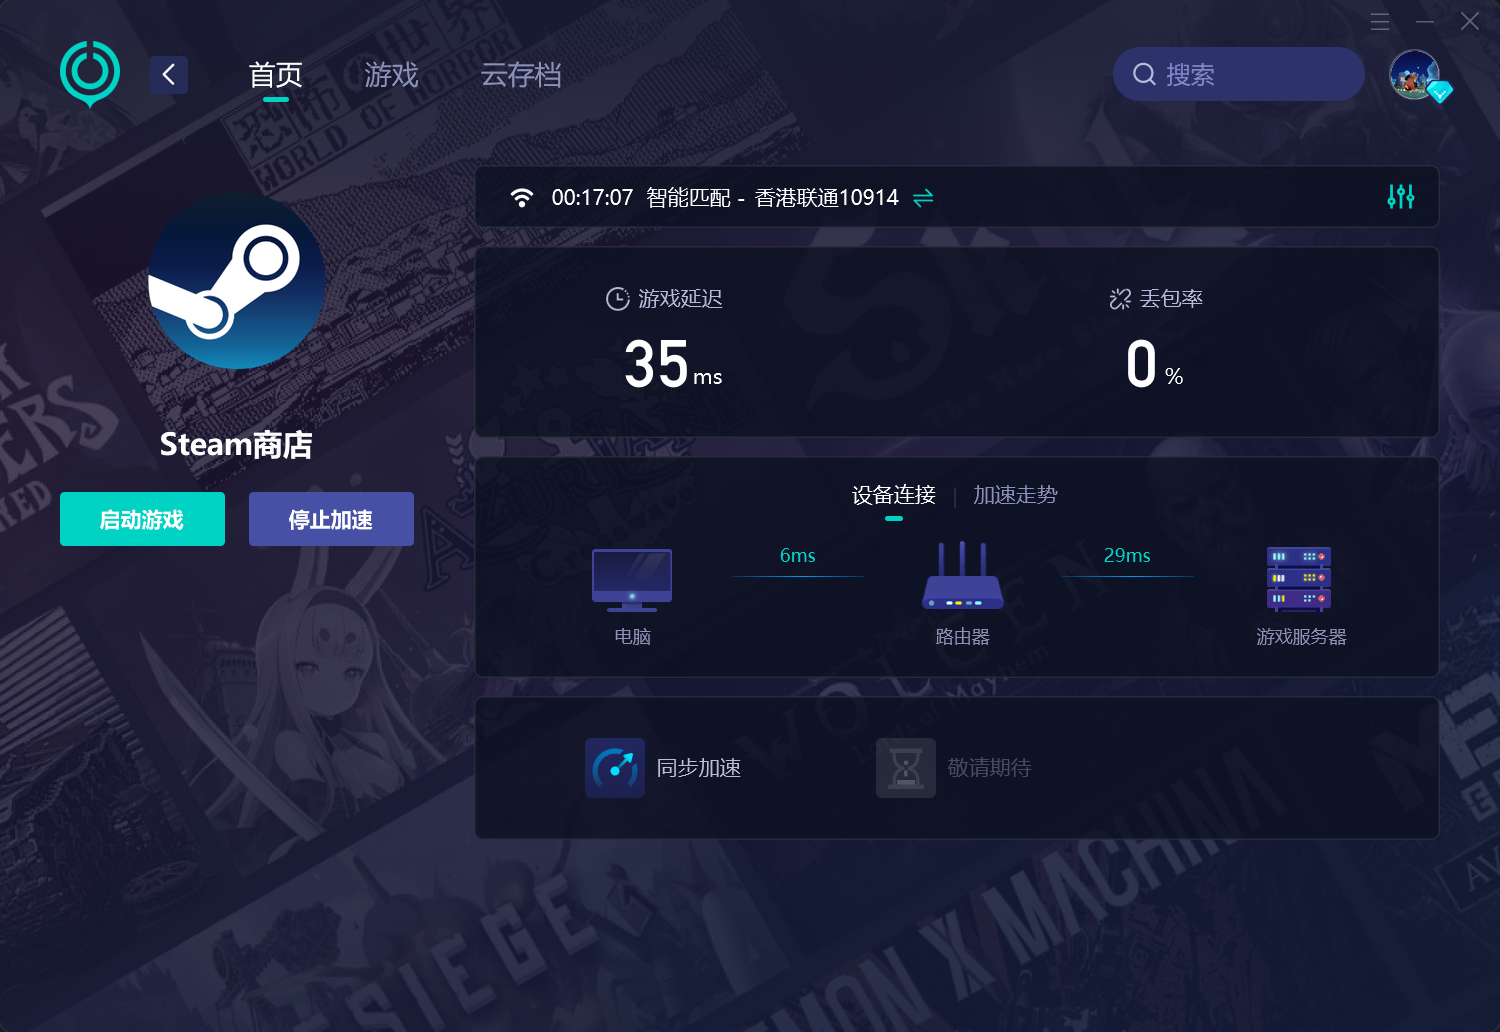
\includegraphics[width=0.7\linewidth]{图/uu加速器.png}
    \caption{\label{fig:uu}Steam加速页面}
    \end{figure}
    \begin{figure}[H]
    \centering
    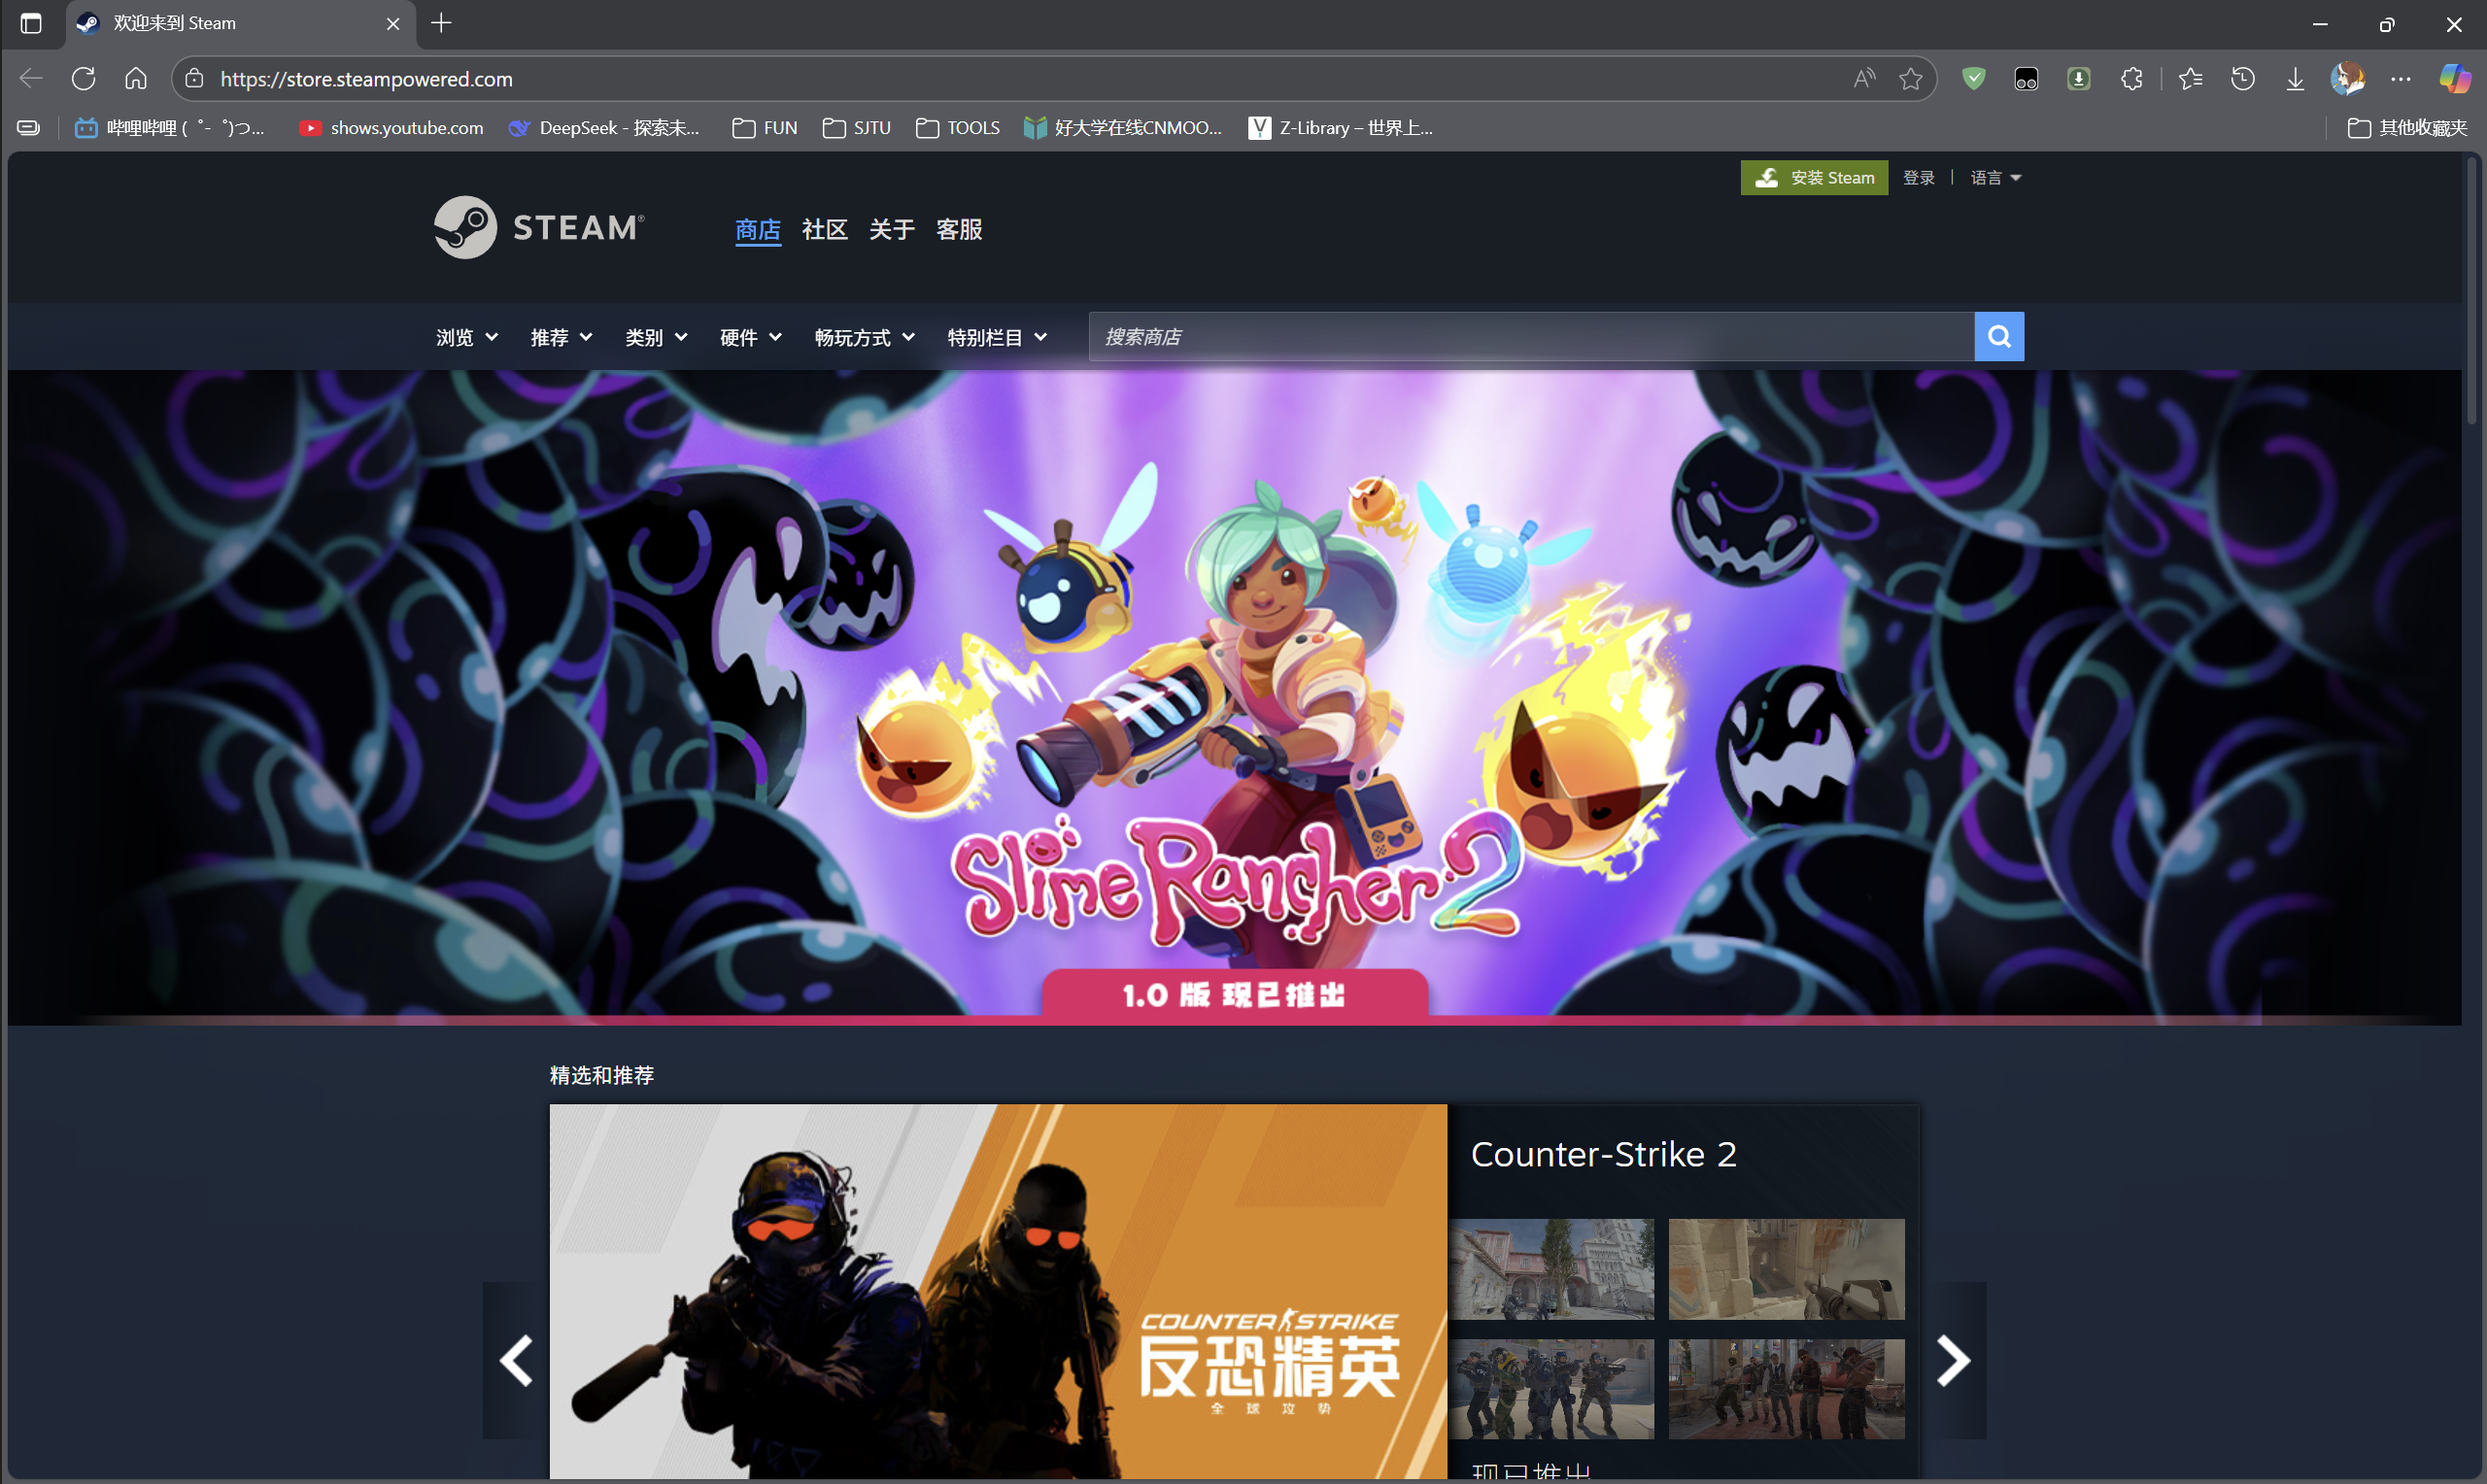
\includegraphics[width=0.7\linewidth]{图/Steam网页.png}
    \caption{\label{fig:Steam正版网页}正版网站界面}
    \end{figure}
    \begin{figure}[H]
    \centering
    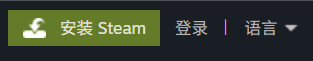
\includegraphics[width=0.7\linewidth]{图/安装图标.png}
    \caption{\label{fig:Steam安装图标}安装图标}
    \end{figure}
    
    \subsubsection{关于蒸汽平台}
    蒸汽平台是国内本土化的Steam,但由于笔者还未体验过,因此不做评价。但就笔者所知,蒸汽平台玩家数量远远不如Steam。推荐大家都去使用Steam而不是蒸汽平台,避免多余麻烦。
    
    \subsection{常见盗版网站和盗版损害}
    上面我们提到了正版Steam的下载,如果各位感兴趣可以去网上看看盗版网页长什么样(笔者由于电脑的广告关闭功能太过完备没有直接在网上搜到素材就不给大家搬运了)。
    
    有的人会说,我下盗版Steam的管你什么事,我还不是照样能玩游戏。的确,盗版Steam短时间可能没有什么问题。但是时间久了以后你就会发现,你的盗版Steam会弹出会员充值项目,商城里的游戏会以更贵的价格卖给你,并且你并不是你账号的唯一拥有者,而是很多人共同使用这一个账号,所以有时候其他人在玩游戏会导致你玩不了,或者玩一半你被踢出去了。相比之下,Steam本身是免费的,游玩体验也远胜盗版,没有必要去折磨自己。

\section{Steam的常见功能}
    \subsection{主页}
    当你登录上你的账户并且打开后看到的就是你的Steam主页\ref{fig:Steam主页}(准确一点说,这个界面其实属于商店,但笔者还是姑且叫它主页)。
    \begin{figure}[H]
    \centering
    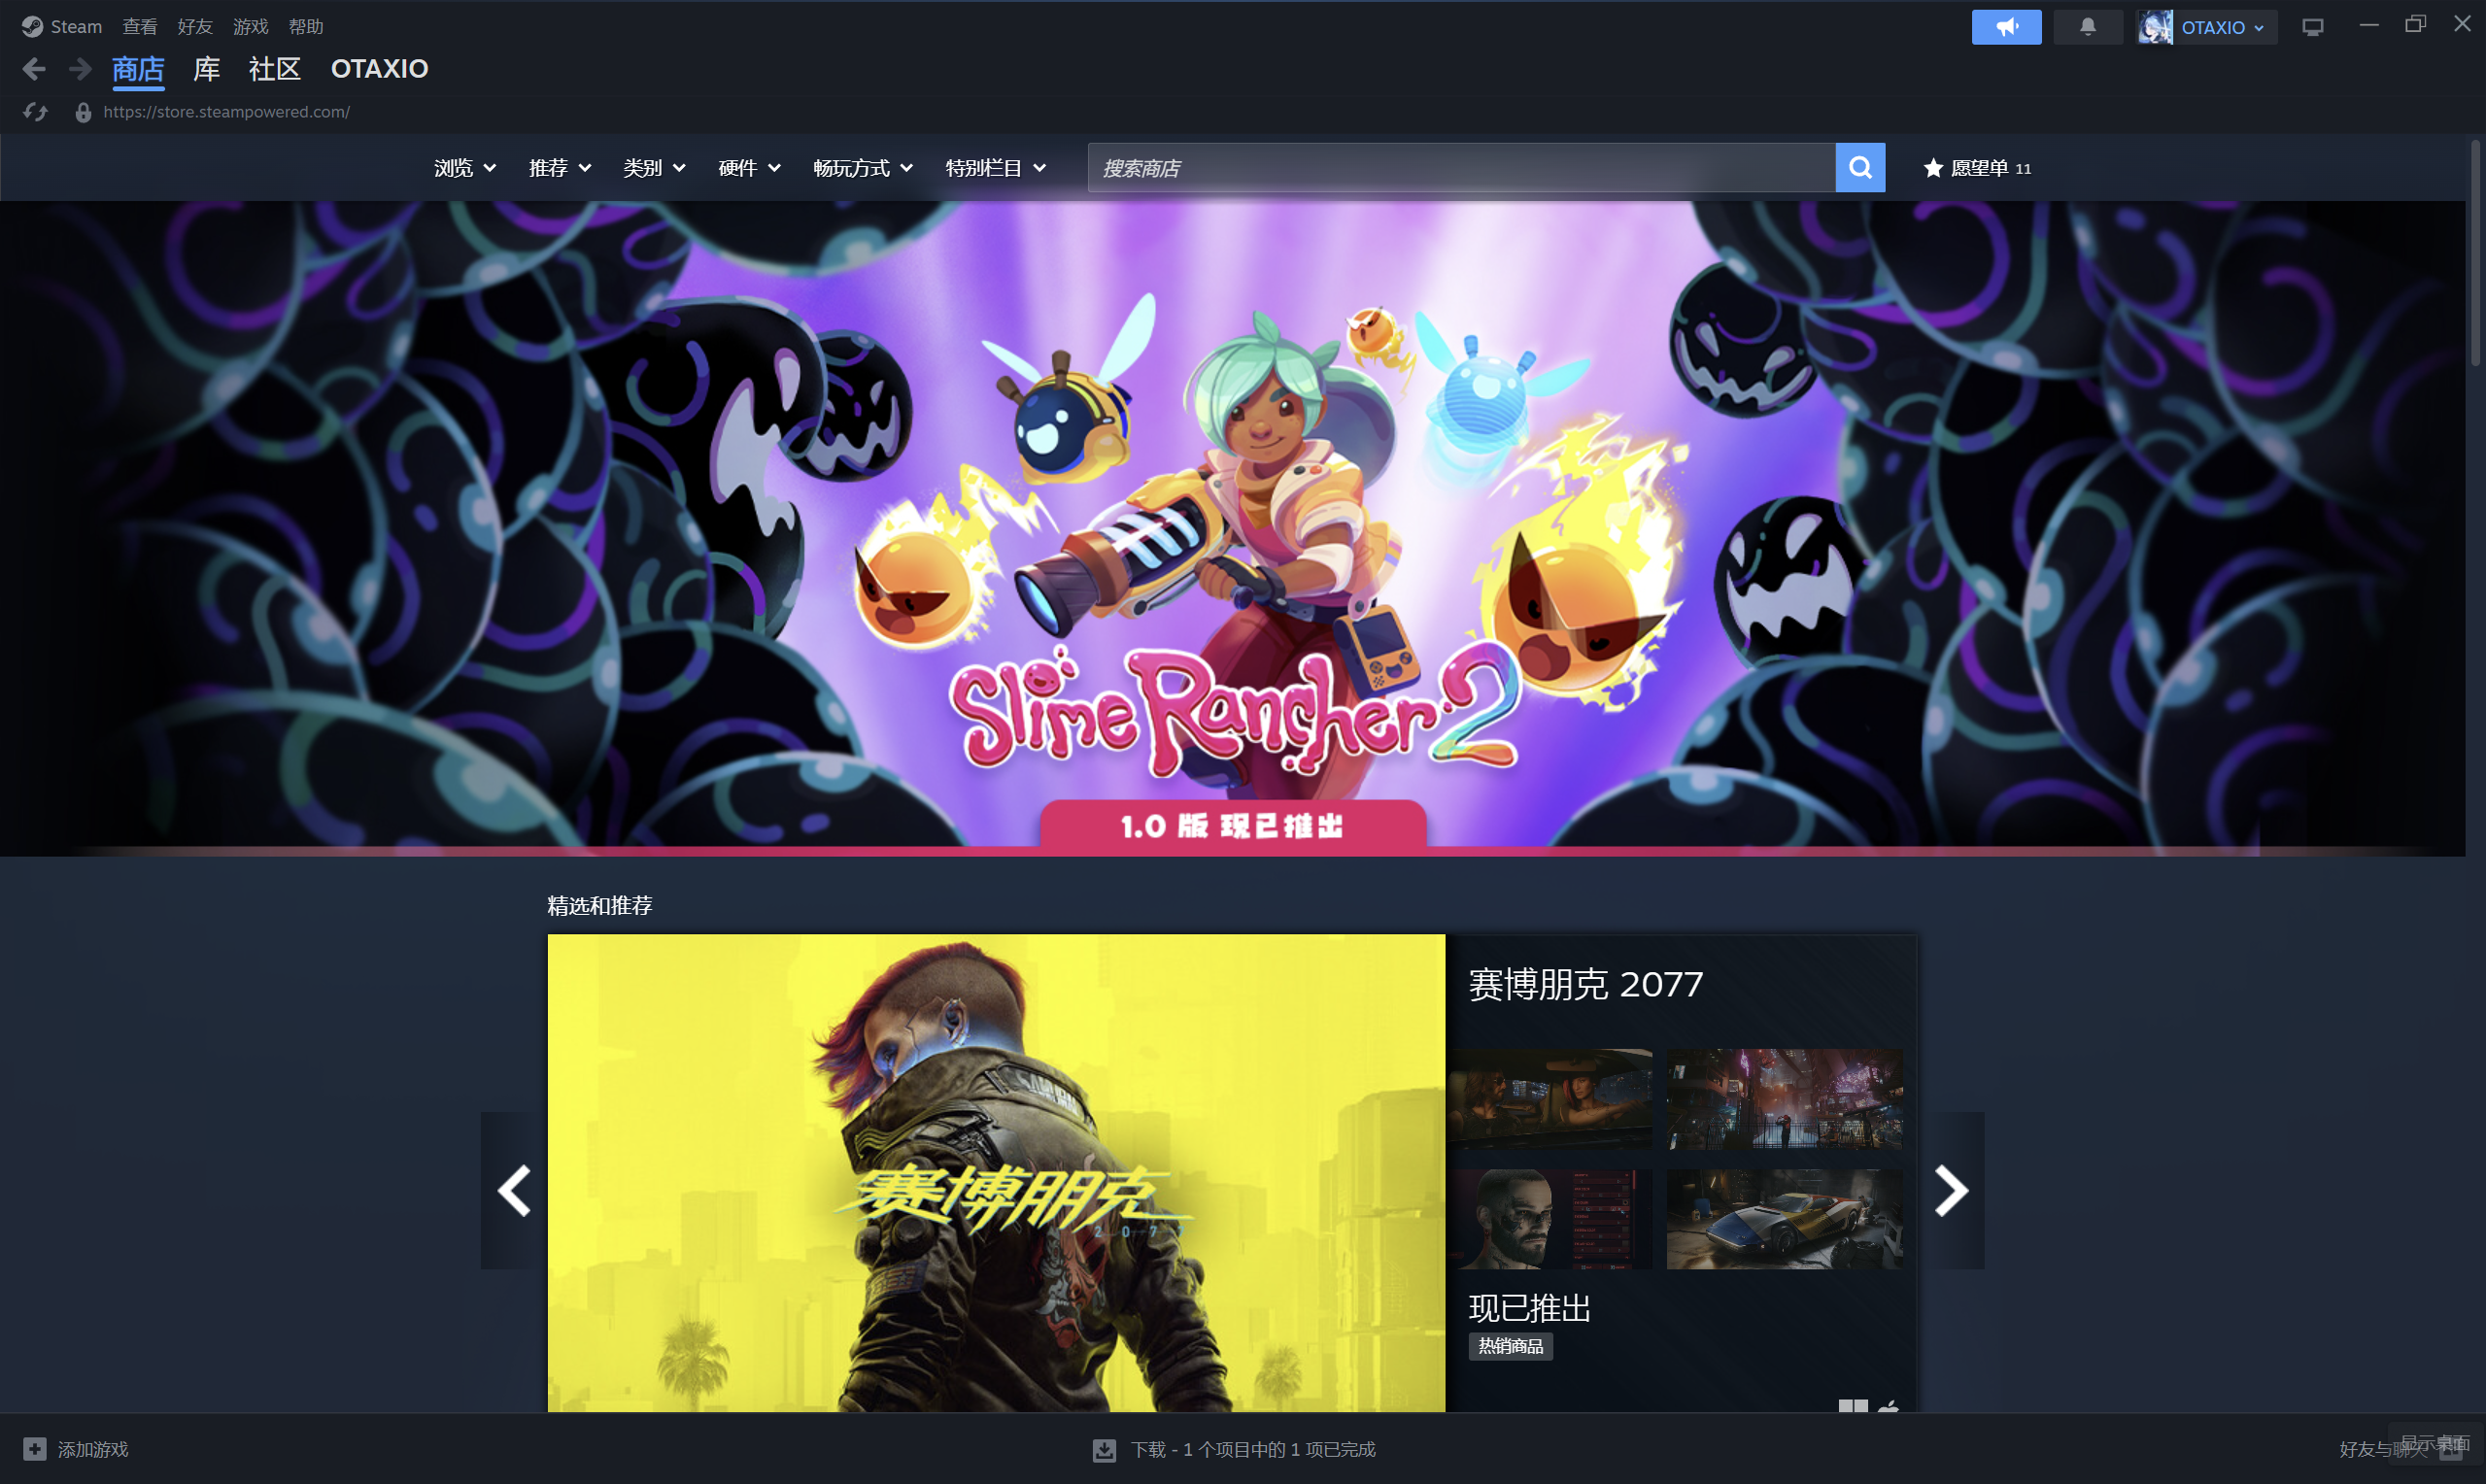
\includegraphics[width=0.7\linewidth]{图/Steam主页.png}
    \caption{\label{fig:Steam主页}Steam主页}
    \end{figure}
    从这个页面往下翻\ref{fig:往下翻},可以看到游戏分类,推荐等等。游戏推荐应该是无穷无尽的,你可以一直往下翻(大概)。
    \begin{figure}[H]
    \centering
    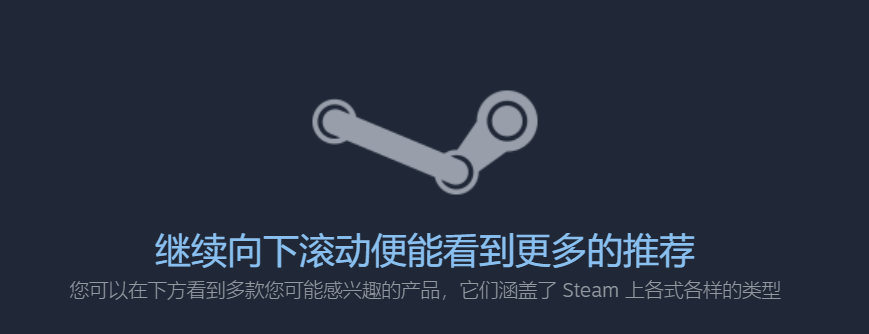
\includegraphics[width=0.7\linewidth]{图/往下翻.png}
    \caption{\label{fig:往下翻}往下翻界面}
    \end{figure}
    笔者在主页使用最多的功能就是找到新品或折扣\ref{fig:折扣与活动},点击右上角的浏览更多,在里面翻看游戏,其他时候主页使用的不多。
    \begin{figure}[H]
    \centering
    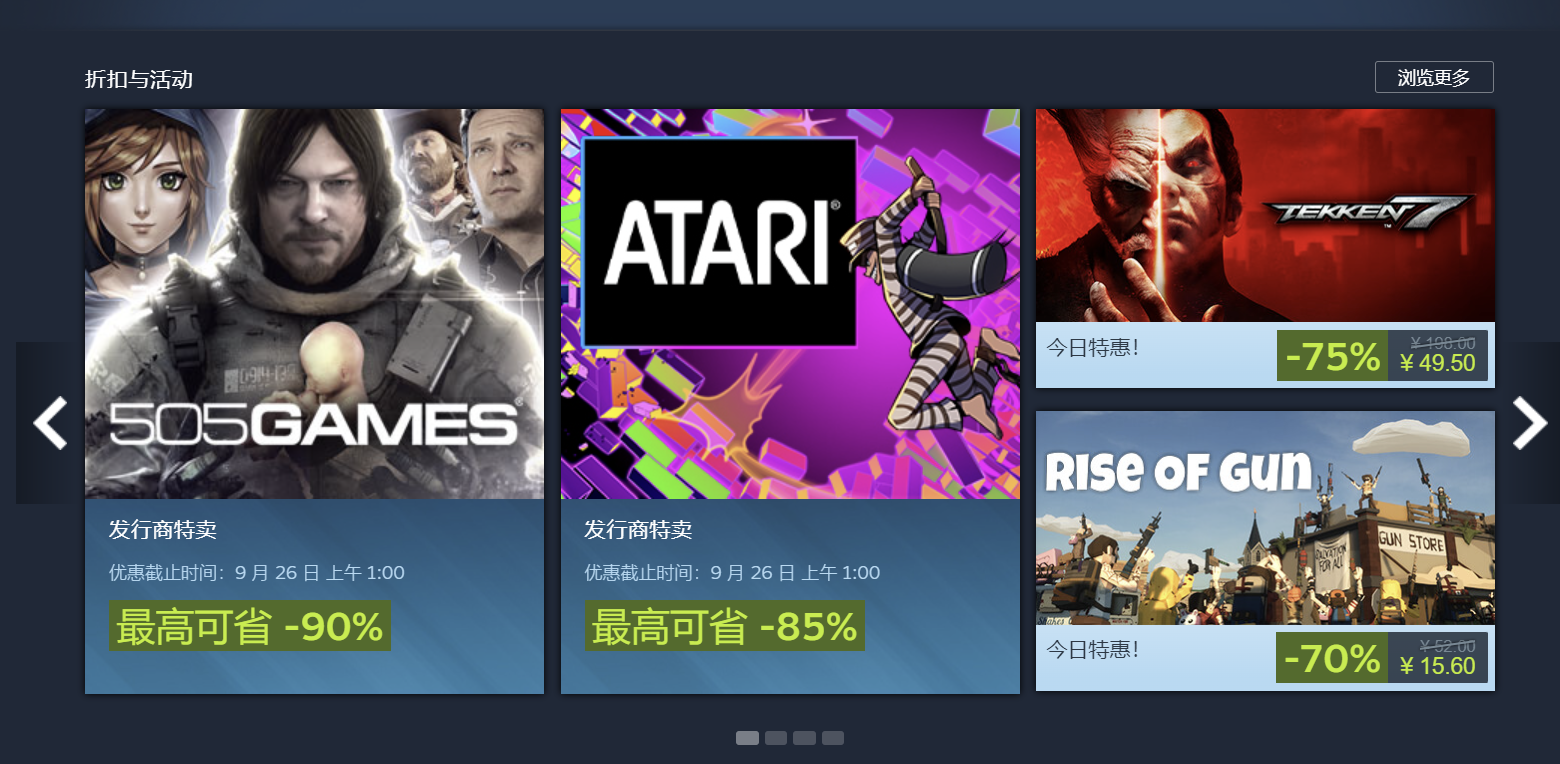
\includegraphics[width=0.7\linewidth]{图/折扣与活动.png}
    \caption{\label{fig:折扣与活动}折扣与活动}
    \end{figure}
    
    \subsection{四大功能}
    然后,我们看看左上角的四个大字号的功能\ref{fig:四大功能}。
    \begin{figure}[H]
    \centering
    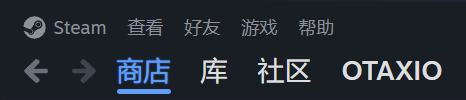
\includegraphics[width=0.7\linewidth]{图/主要四功能.png}
    \caption{\label{fig:四大功能}Steam四大功能}
    \end{figure}
    这四个功能分别是商店,库,社区,OTAXIO(你的用户名称)。下面笔者将详细介绍这四大功能。
        \subsubsection{商店}
        顾名思义,商店就是你在Steam上购买游戏的地方,在主页你点击游戏跳转到的页面也属于商店。然而,在Steam上买游戏并不只有在Steam商城购买这一种方式,在后面会有专门的篇章讲解Steam游戏的购买渠道。
        
        将鼠标放在商店这个按钮上,你会看到精选,探索队列,愿望单,点数商店,新闻和统计数据六个分区。
        \begin{itemize}
            \item 精选\ref{fig:精选}其实就是主页\ref{fig:Steam主页},是Steam官方的游戏推荐,基本上会包含最近打折的游戏,新出的游戏和最近热门的游戏,没事可以在这个界面逛逛。
            \item 探索队列\ref{fig:探索队列}则是根据你平时游玩的游戏类型进行推荐,更加个性化,不过笔者用的很少便不过多介绍了。
            \item 愿望单\ref{fig:愿望单}类似于你在购物平台的收藏,当你把你想要的游戏添加到愿望单以后,你的好友就能够看到你想要哪些游戏(别人可能给你惊喜送你一个),并且当你愿望单里的游戏打折的时候会通过你Steam绑定的邮箱给你发送消息,告诉你你感兴趣的游戏打折了。
            \item 点数商店\ref{fig:点数商店}售卖的主要是Steam上的外观饰品,比如头像,头像框,名片背景,个人资料背景,Steam启动动画等等。点数主要通过购买游戏获得,每在商城花费1美元可以获得10点数。部分饰品需要你拥有对应游戏才能购买,部分饰品会在一些游戏节赠送。
            \item 新闻\ref{fig:新闻中心}就是最近游戏公司等发布的游戏资讯,游戏更新之类的,不过笔者用的很少便不过多介绍了。
            \item 最后是统计数据\ref{fig:统计数据},这上面会展示最近的畅销游戏以及在线人数最多的游戏,感兴趣可以看看。
        \end{itemize}
        \begin{figure}[H]
            \centering
            \begin{minipage}{0.48\textwidth}
                \centering
                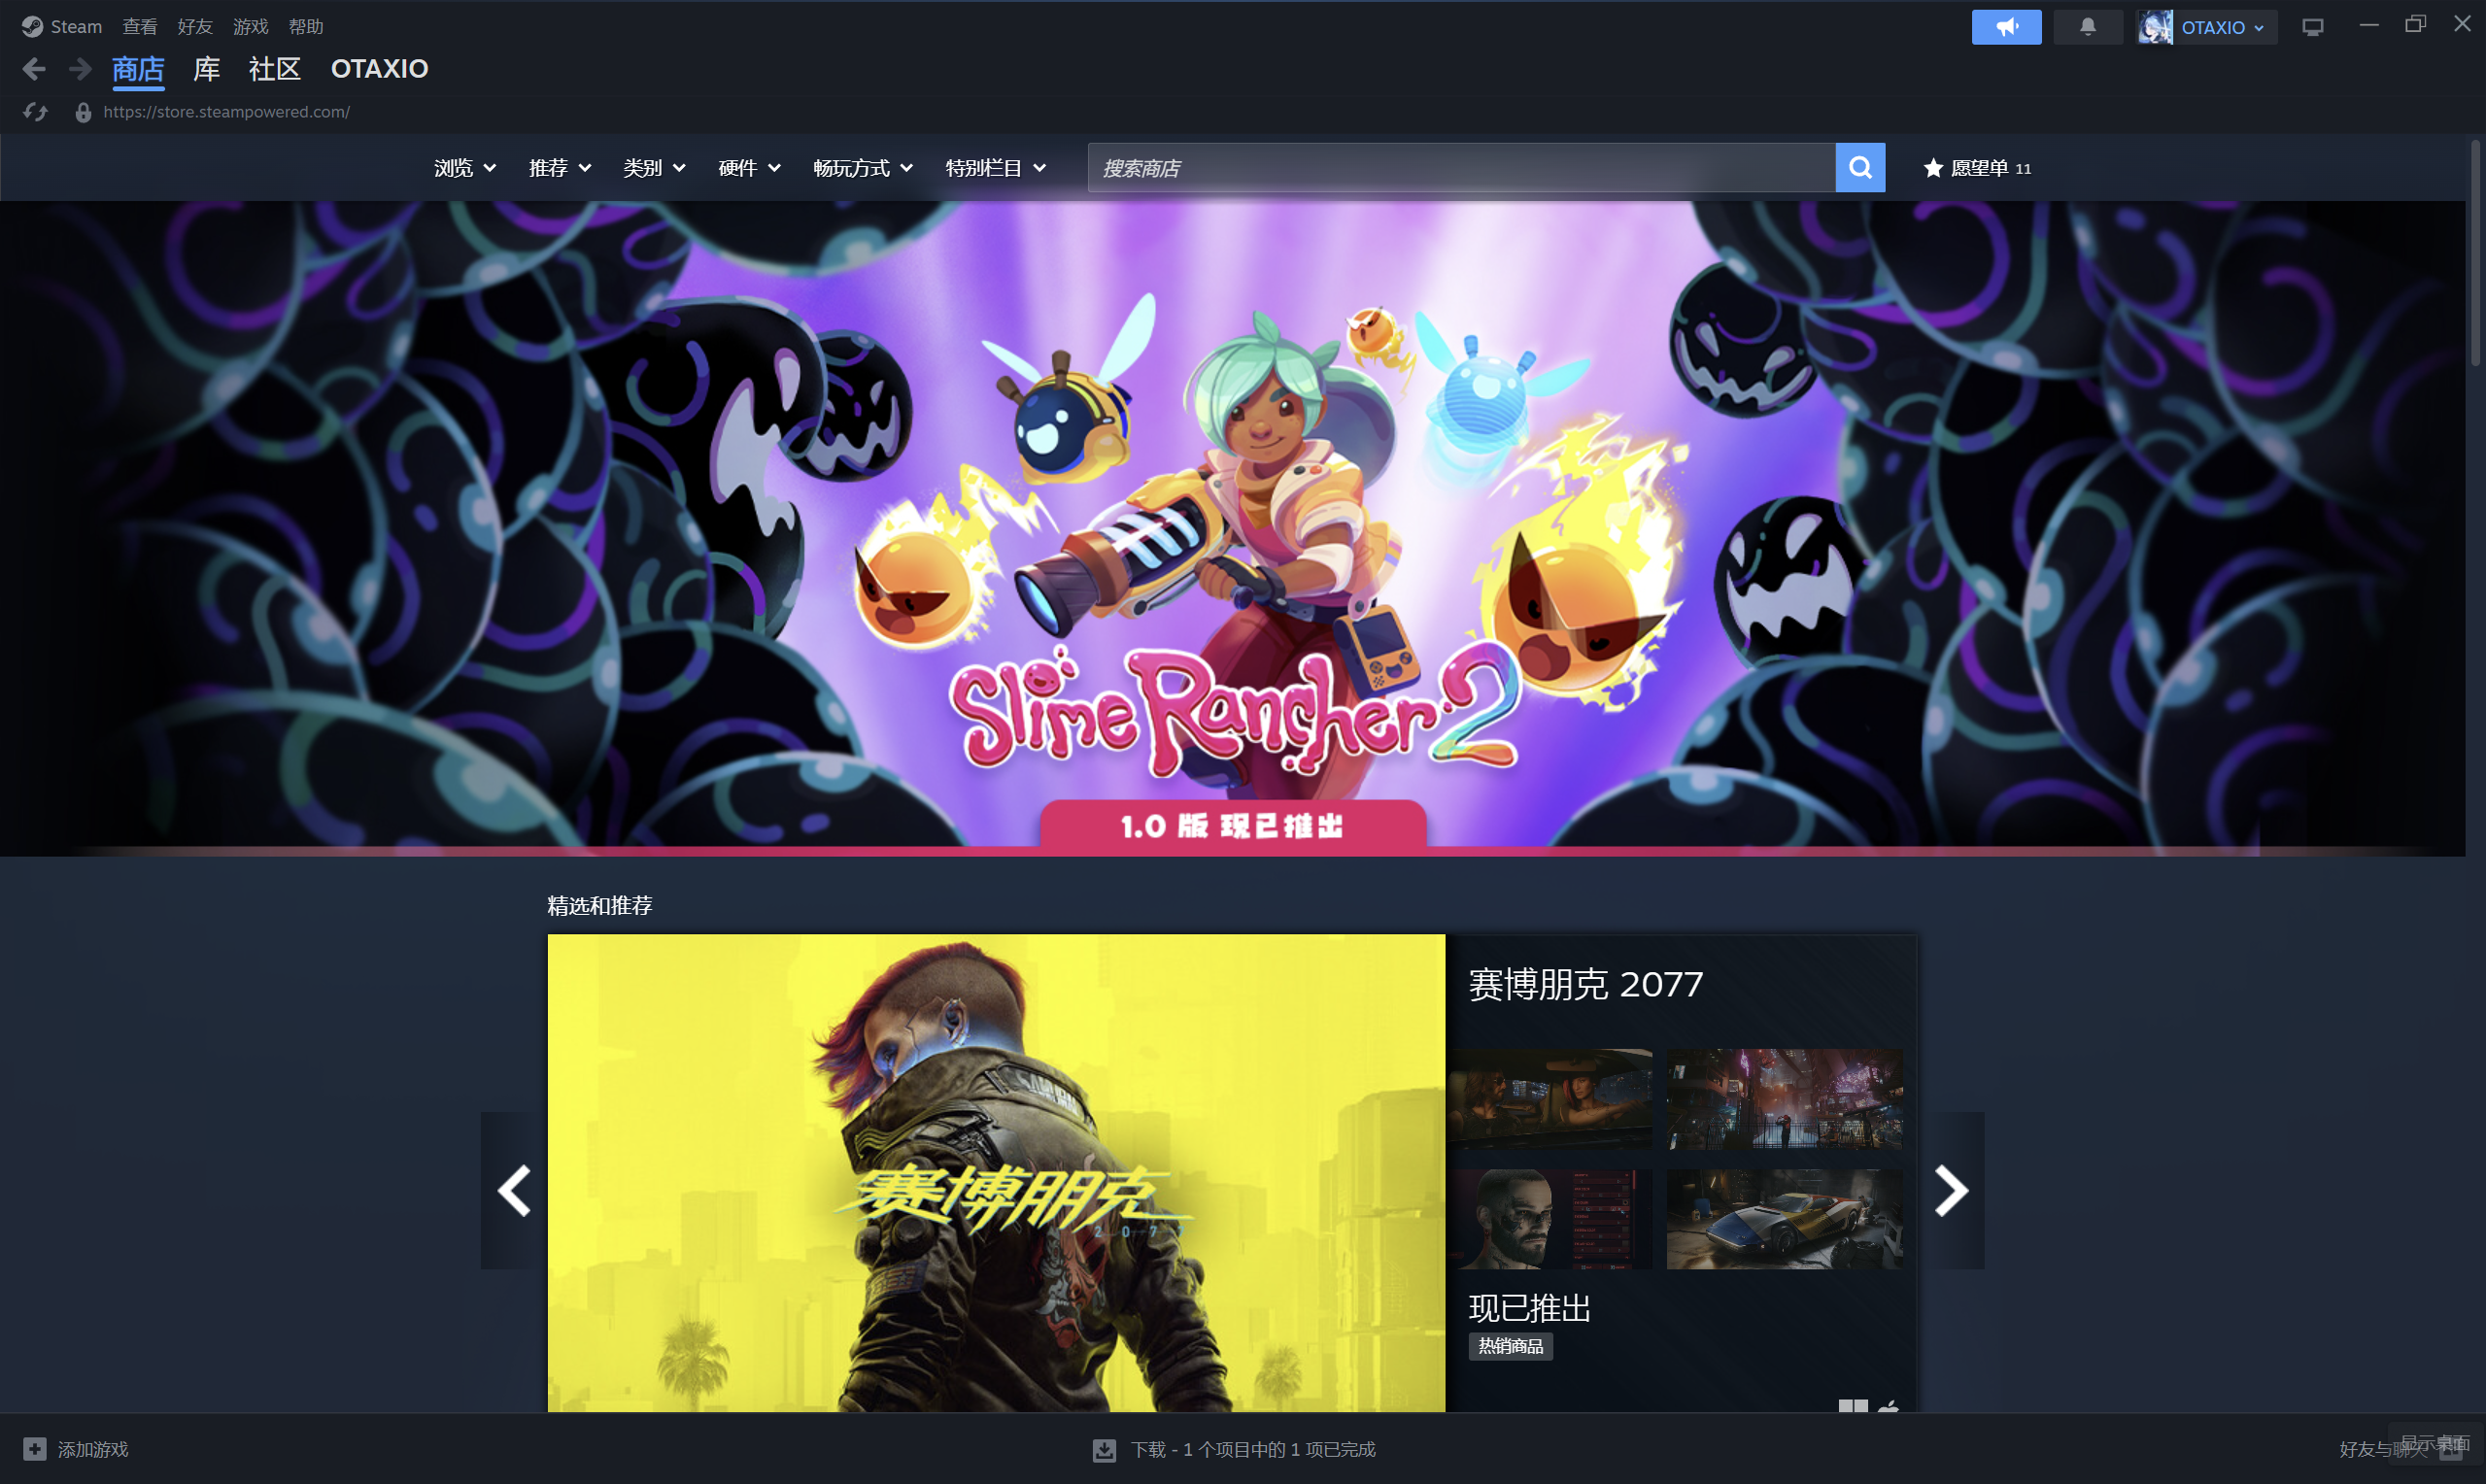
\includegraphics[width=\linewidth]{图/Steam主页.png}
                \caption{精选}
                \label{fig:精选}
            \end{minipage}
            \hfill
            \begin{minipage}{0.48\textwidth}
                \centering
                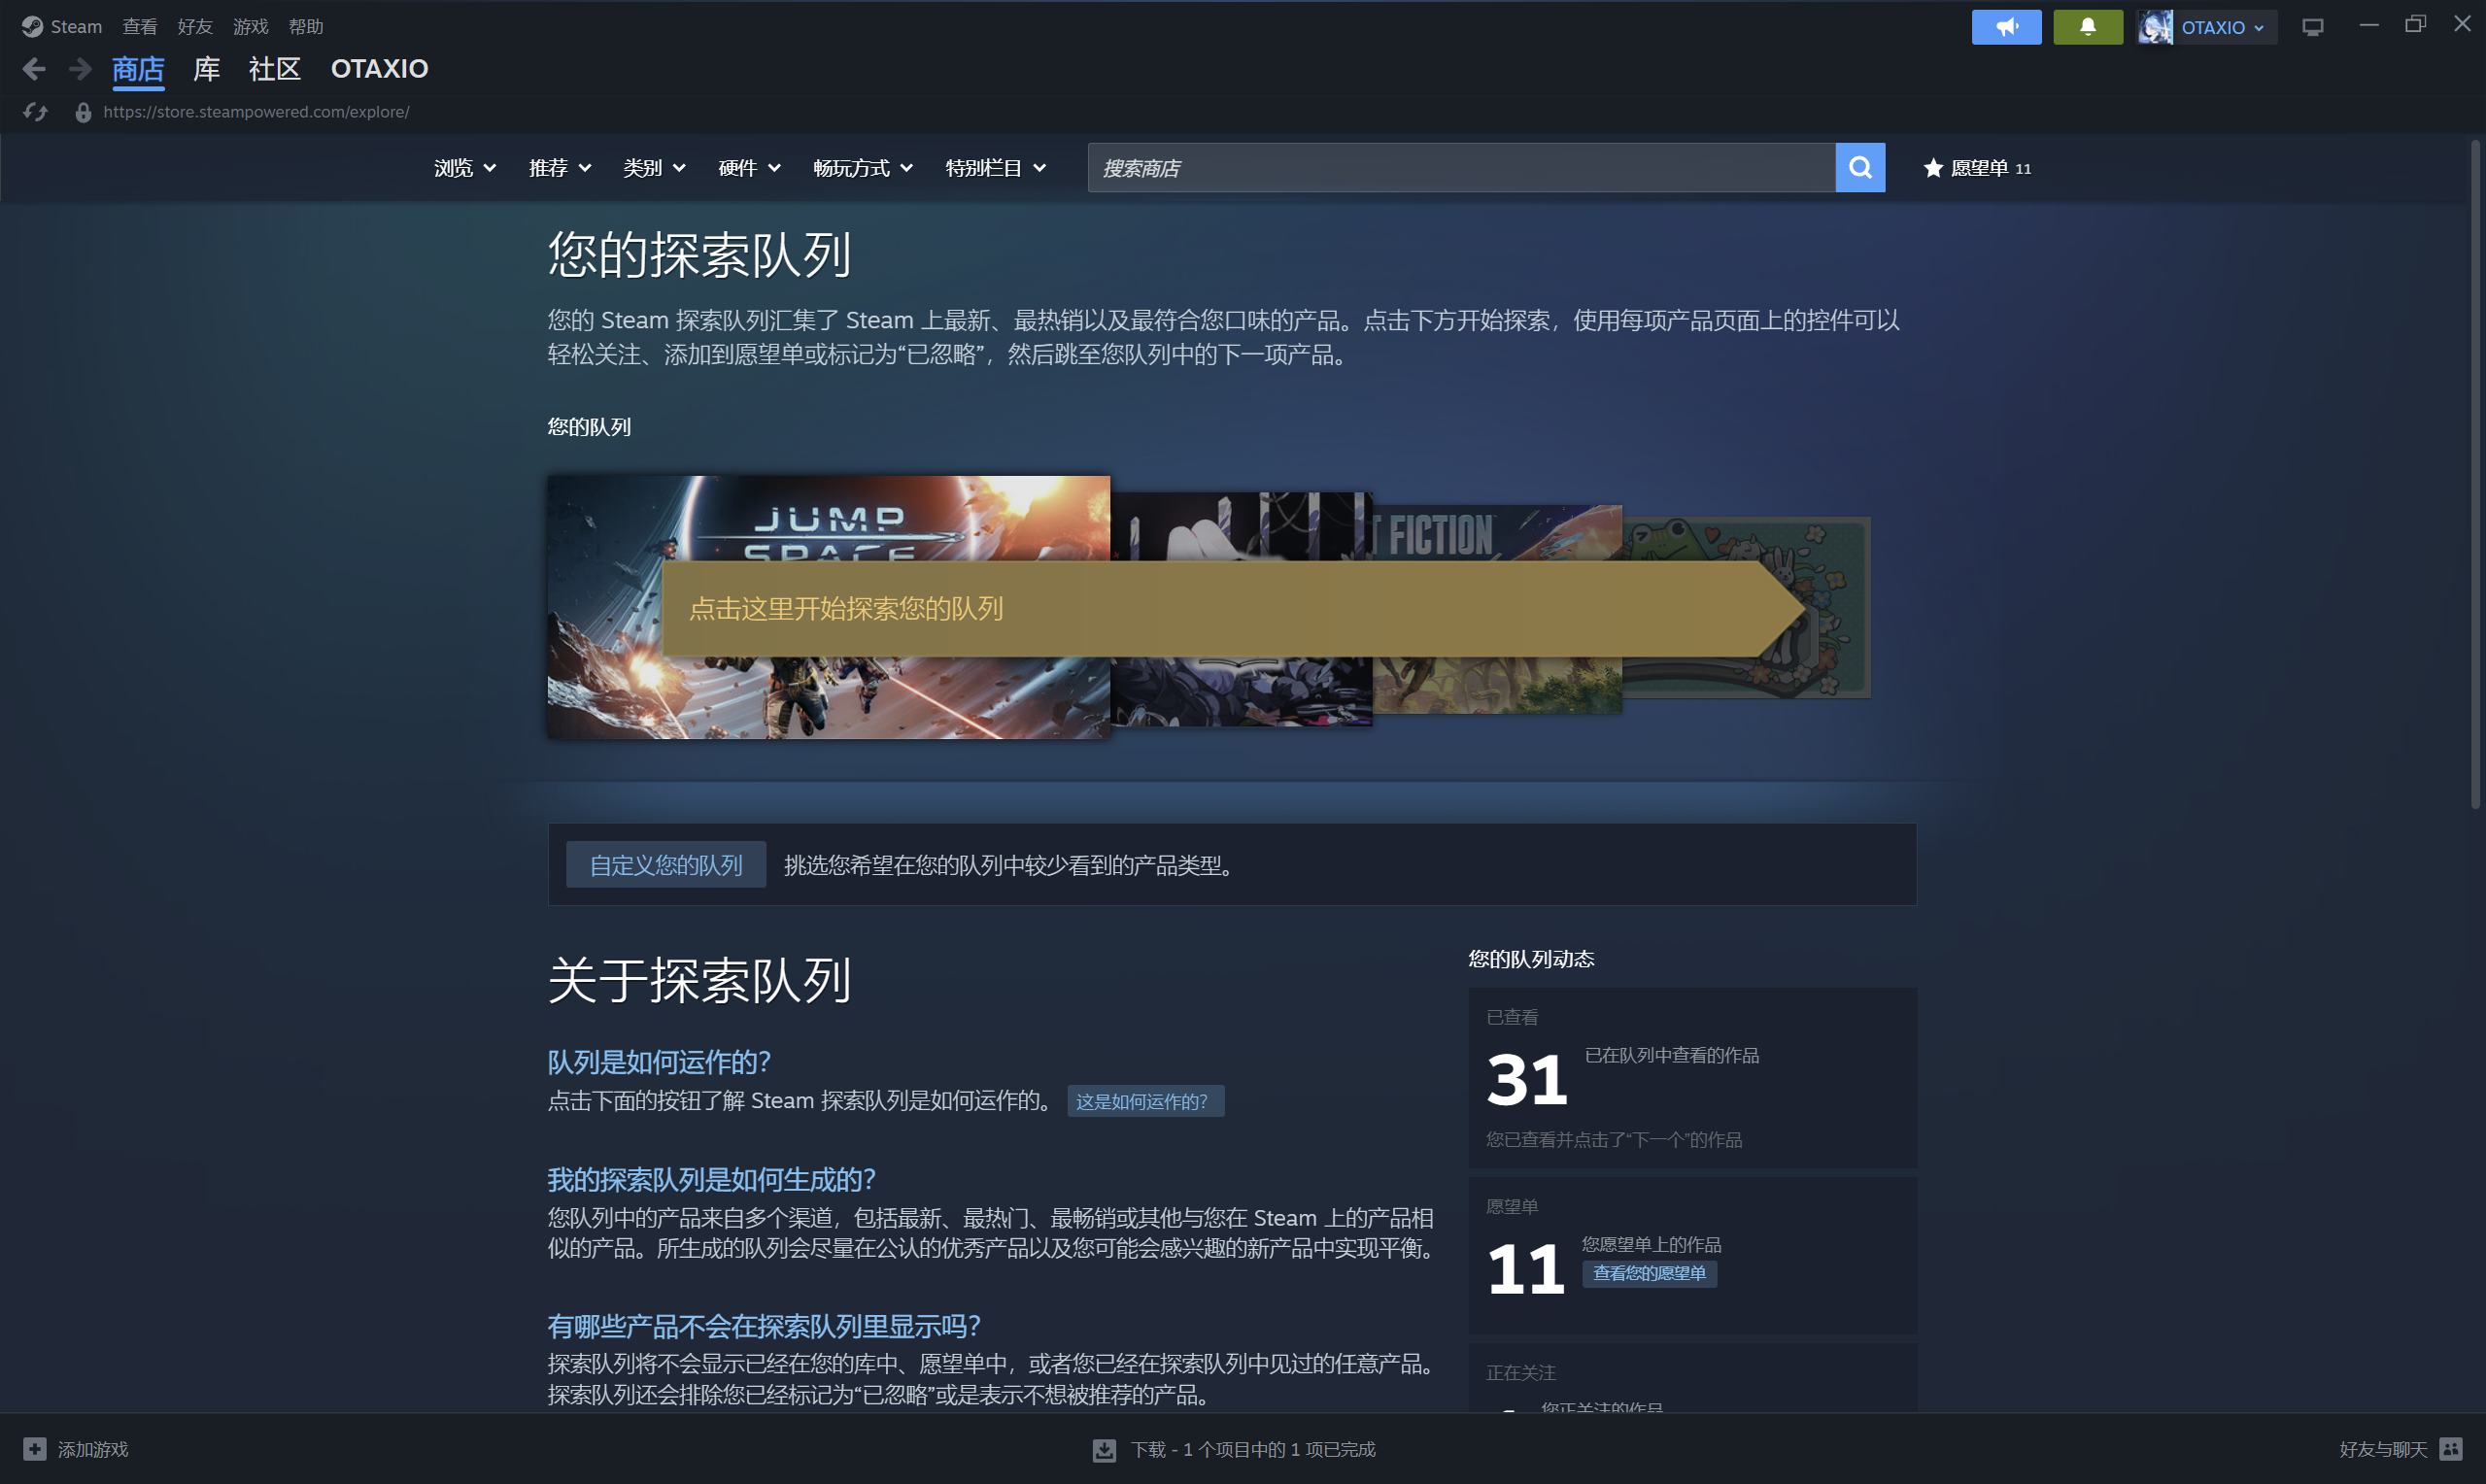
\includegraphics[width=\linewidth]{图/探索队列.png}
                \caption{探索队列}
                \label{fig:探索队列}
            \end{minipage}
        \end{figure}
        
        \begin{figure}[H]
            \centering
            \begin{minipage}{0.48\textwidth}
                \centering
                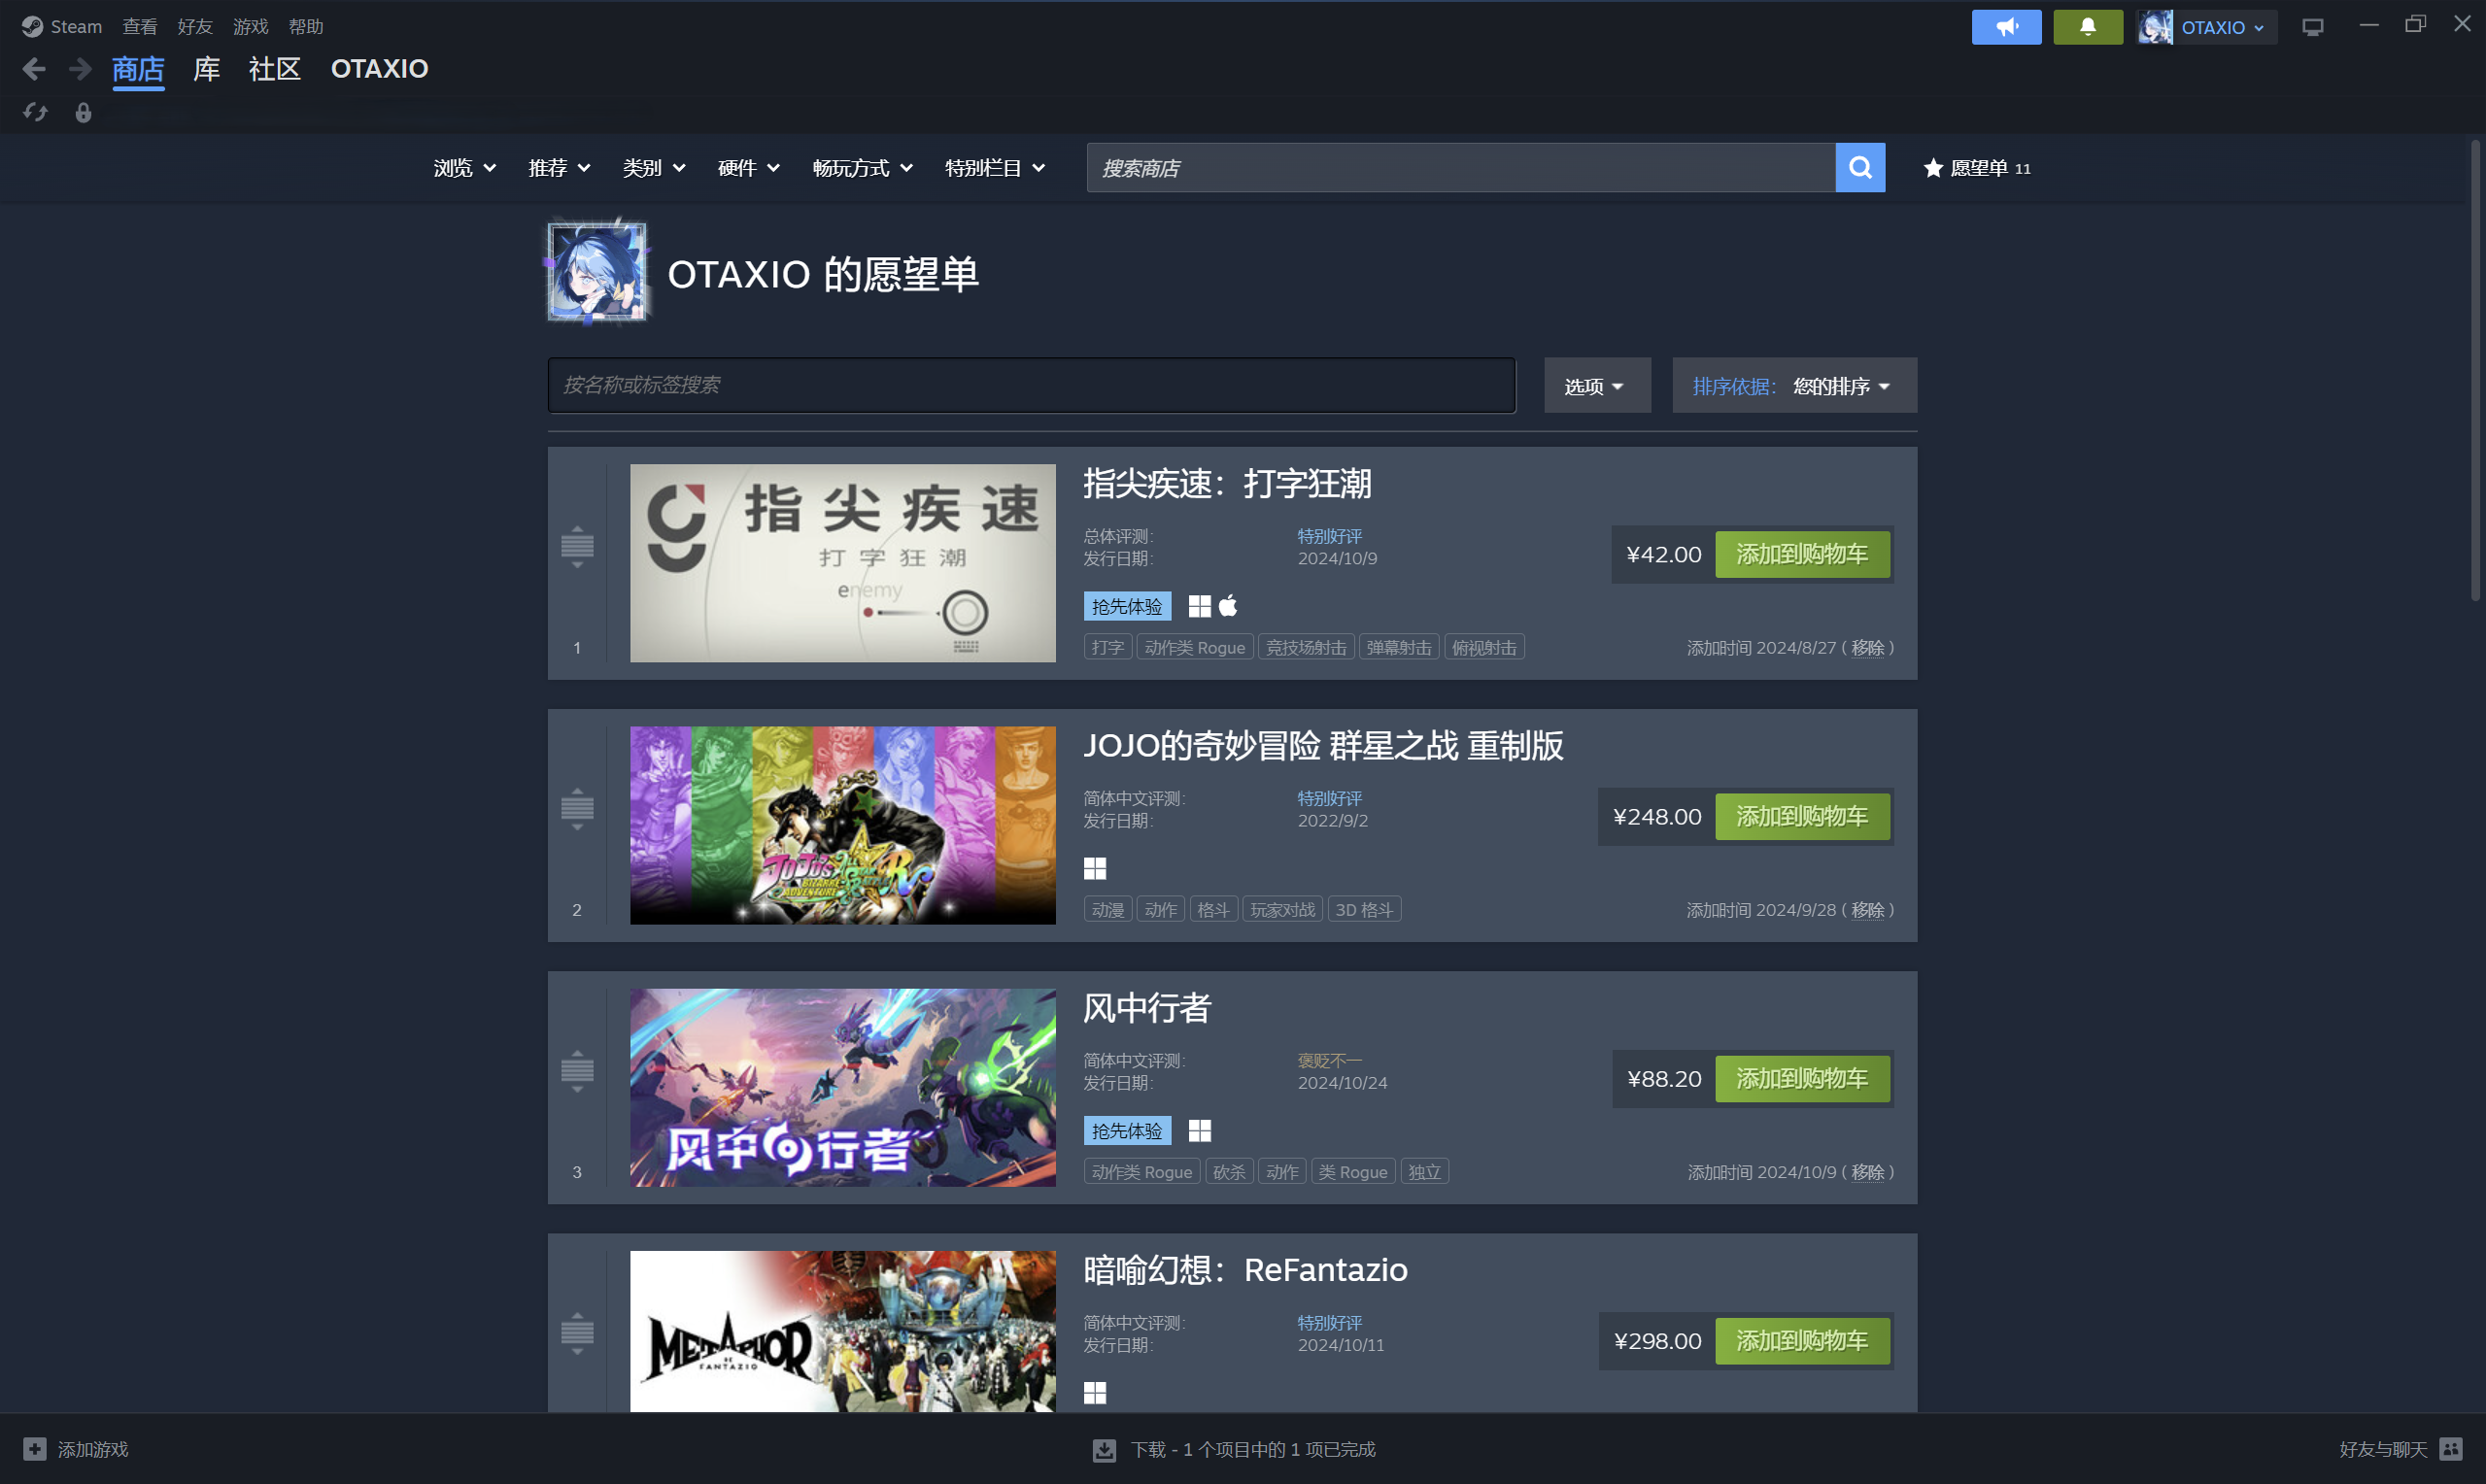
\includegraphics[width=\linewidth]{图/愿望单.png}
                \caption{愿望单}
                \label{fig:愿望单}
            \end{minipage}
            \hfill
            \begin{minipage}{0.48\textwidth}
                \centering
                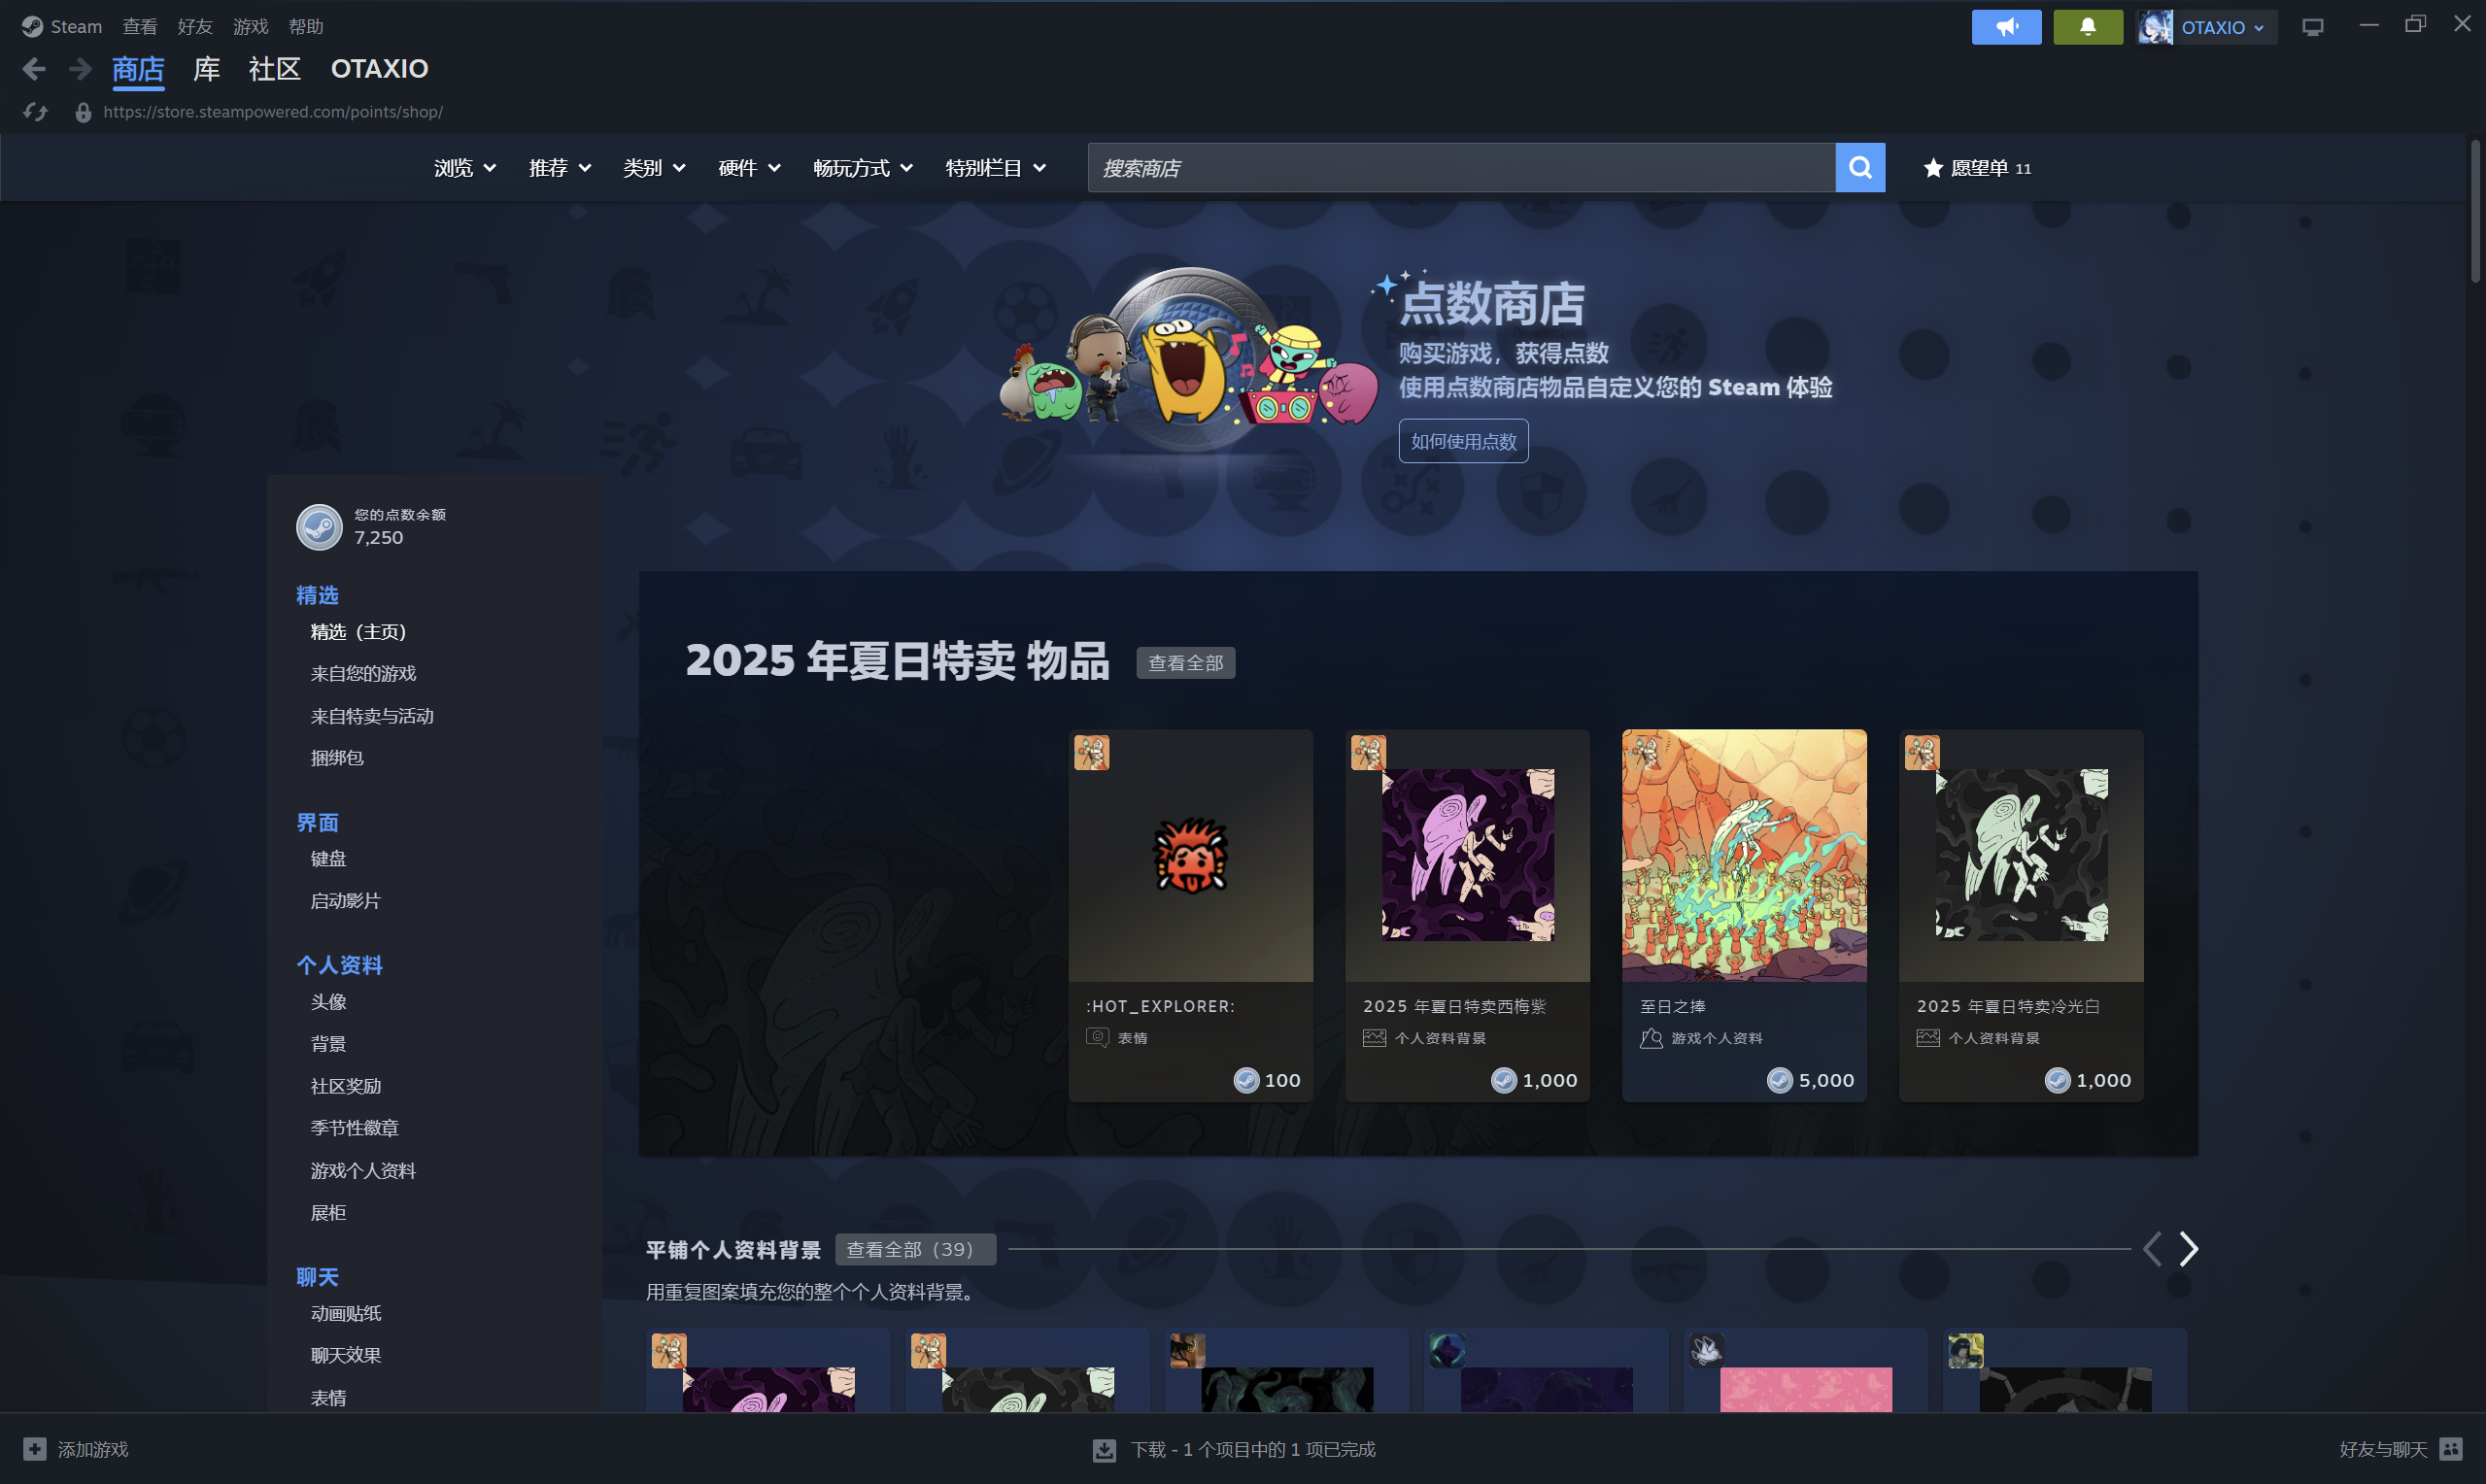
\includegraphics[width=\linewidth]{图/点数商店.png}
                \caption{点数商店}
                \label{fig:点数商店}
            \end{minipage}
        \end{figure}
        
        \begin{figure}[H]
            \centering
            \begin{minipage}{0.48\textwidth}
                \centering
                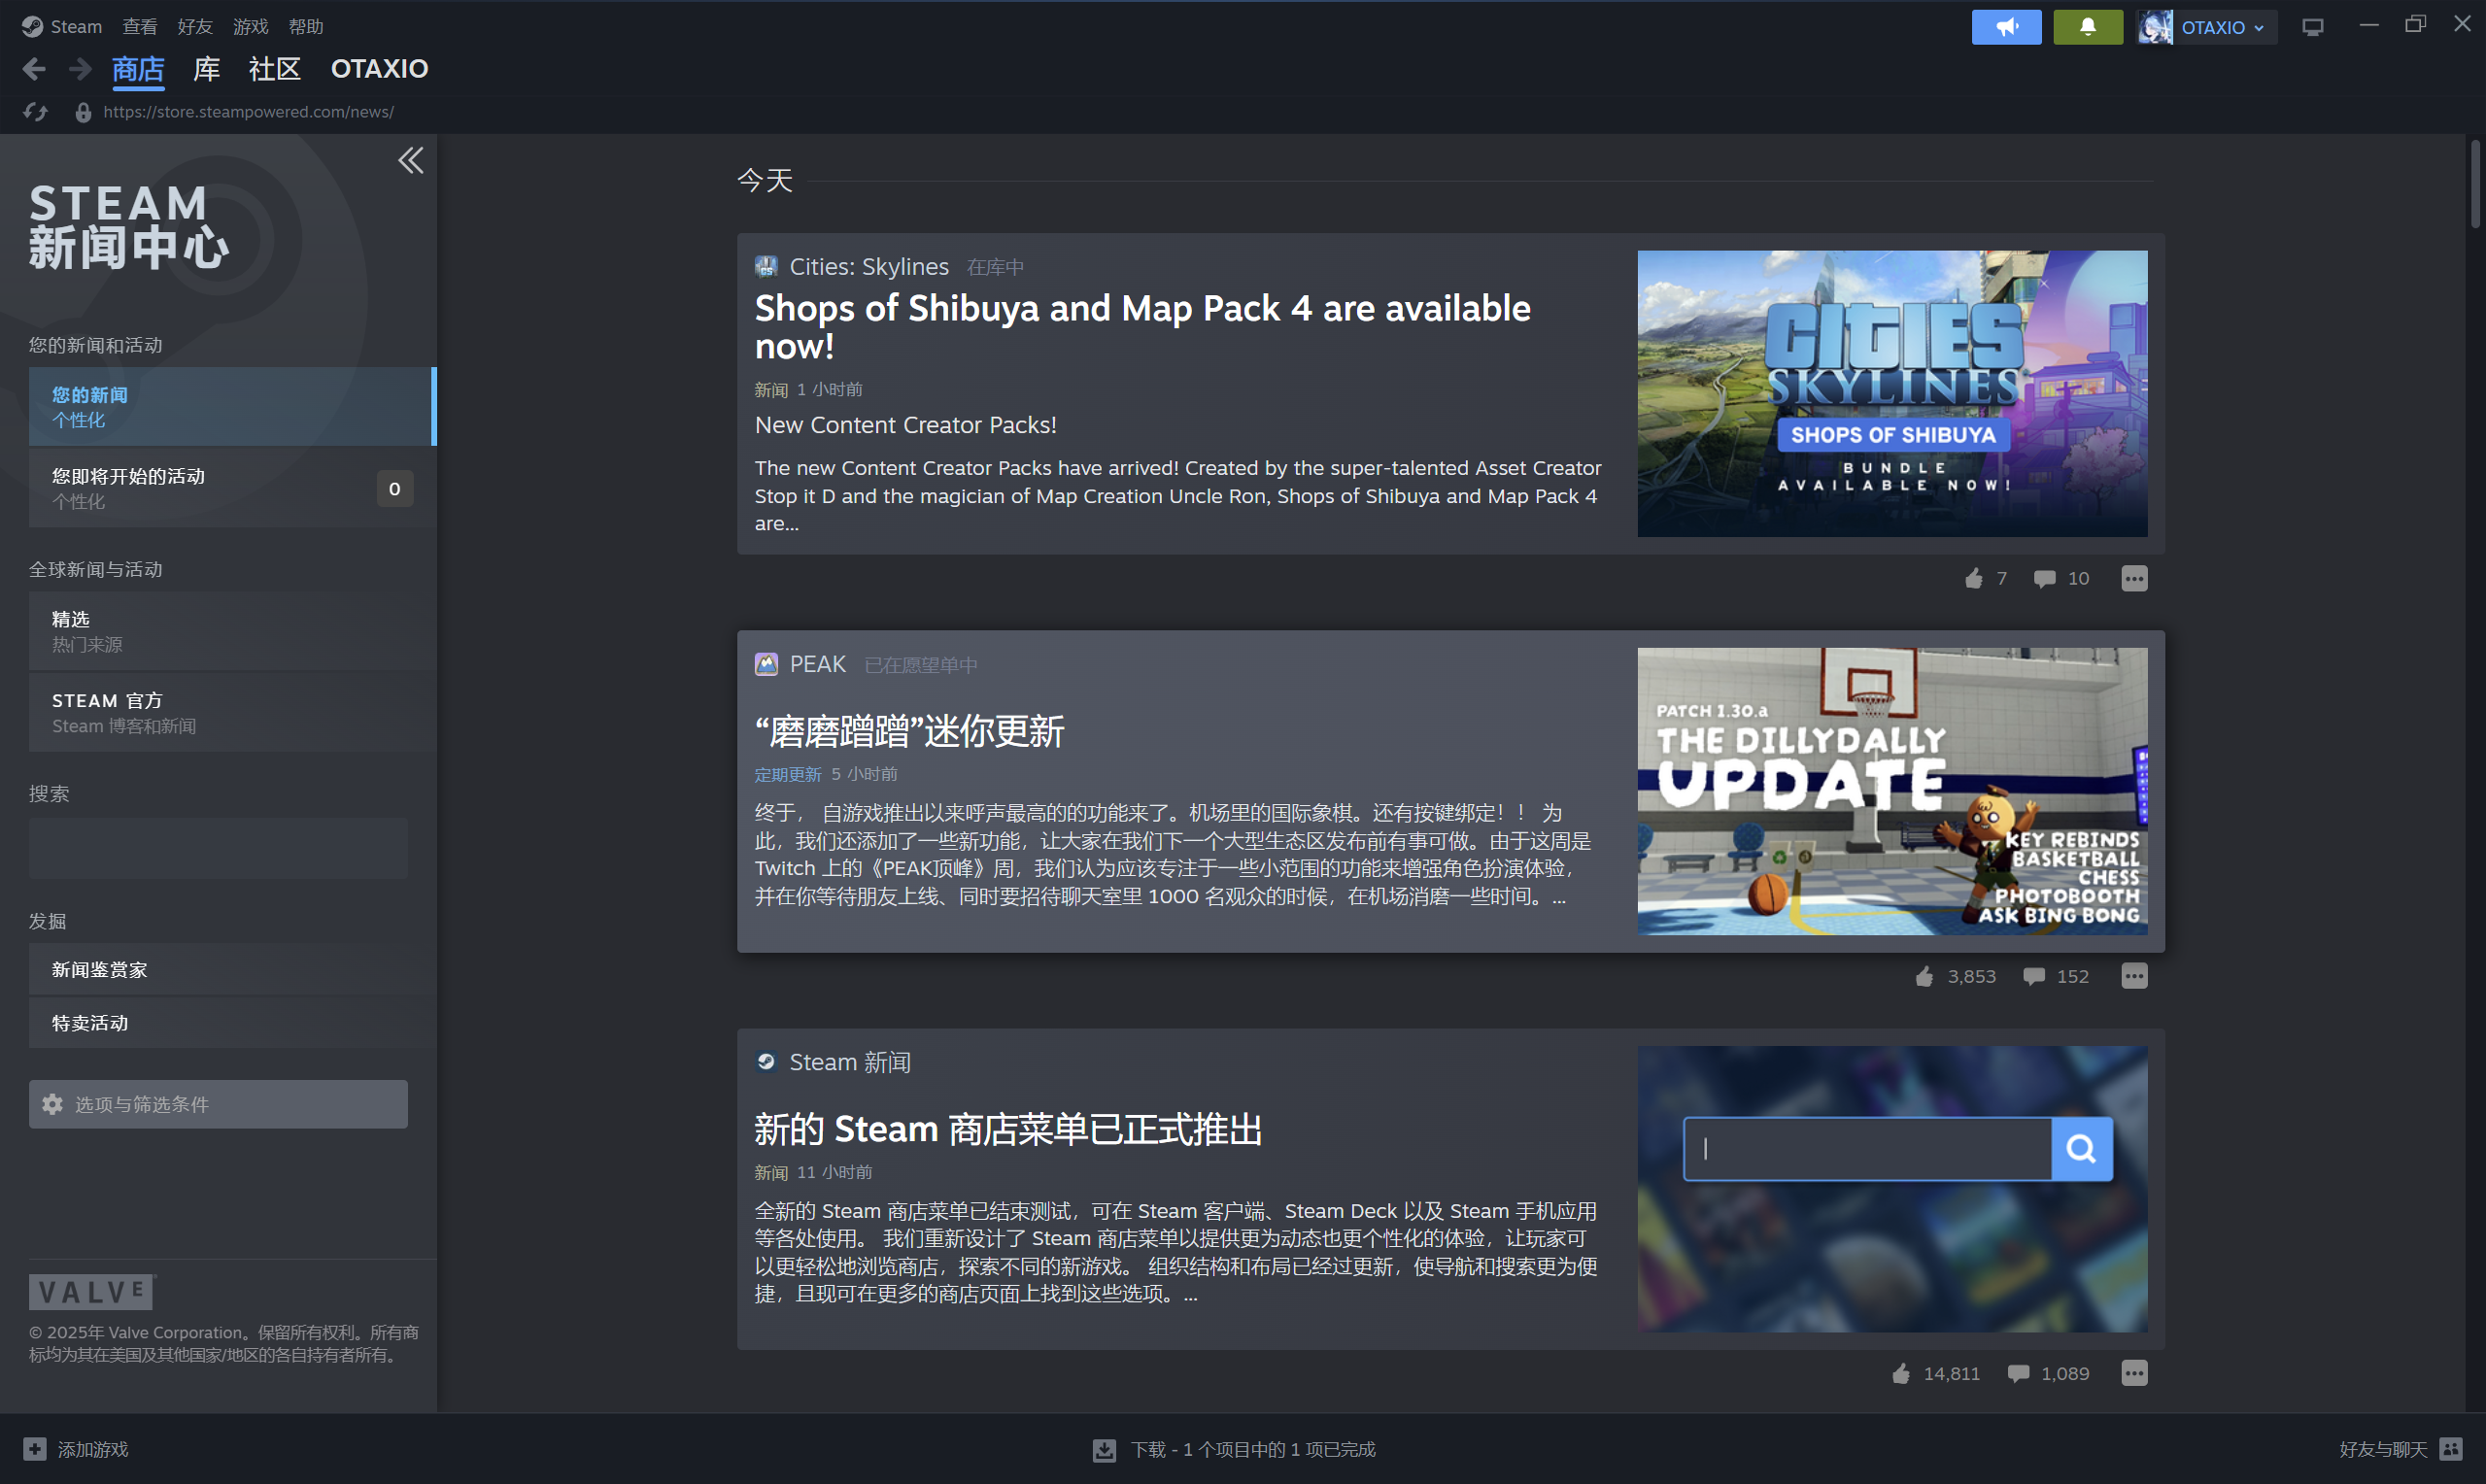
\includegraphics[width=\linewidth]{图/新闻中心.png}
                \caption{新闻}
                \label{fig:新闻中心}
            \end{minipage}
            \hfill
            \begin{minipage}{0.48\textwidth}
                \centering
                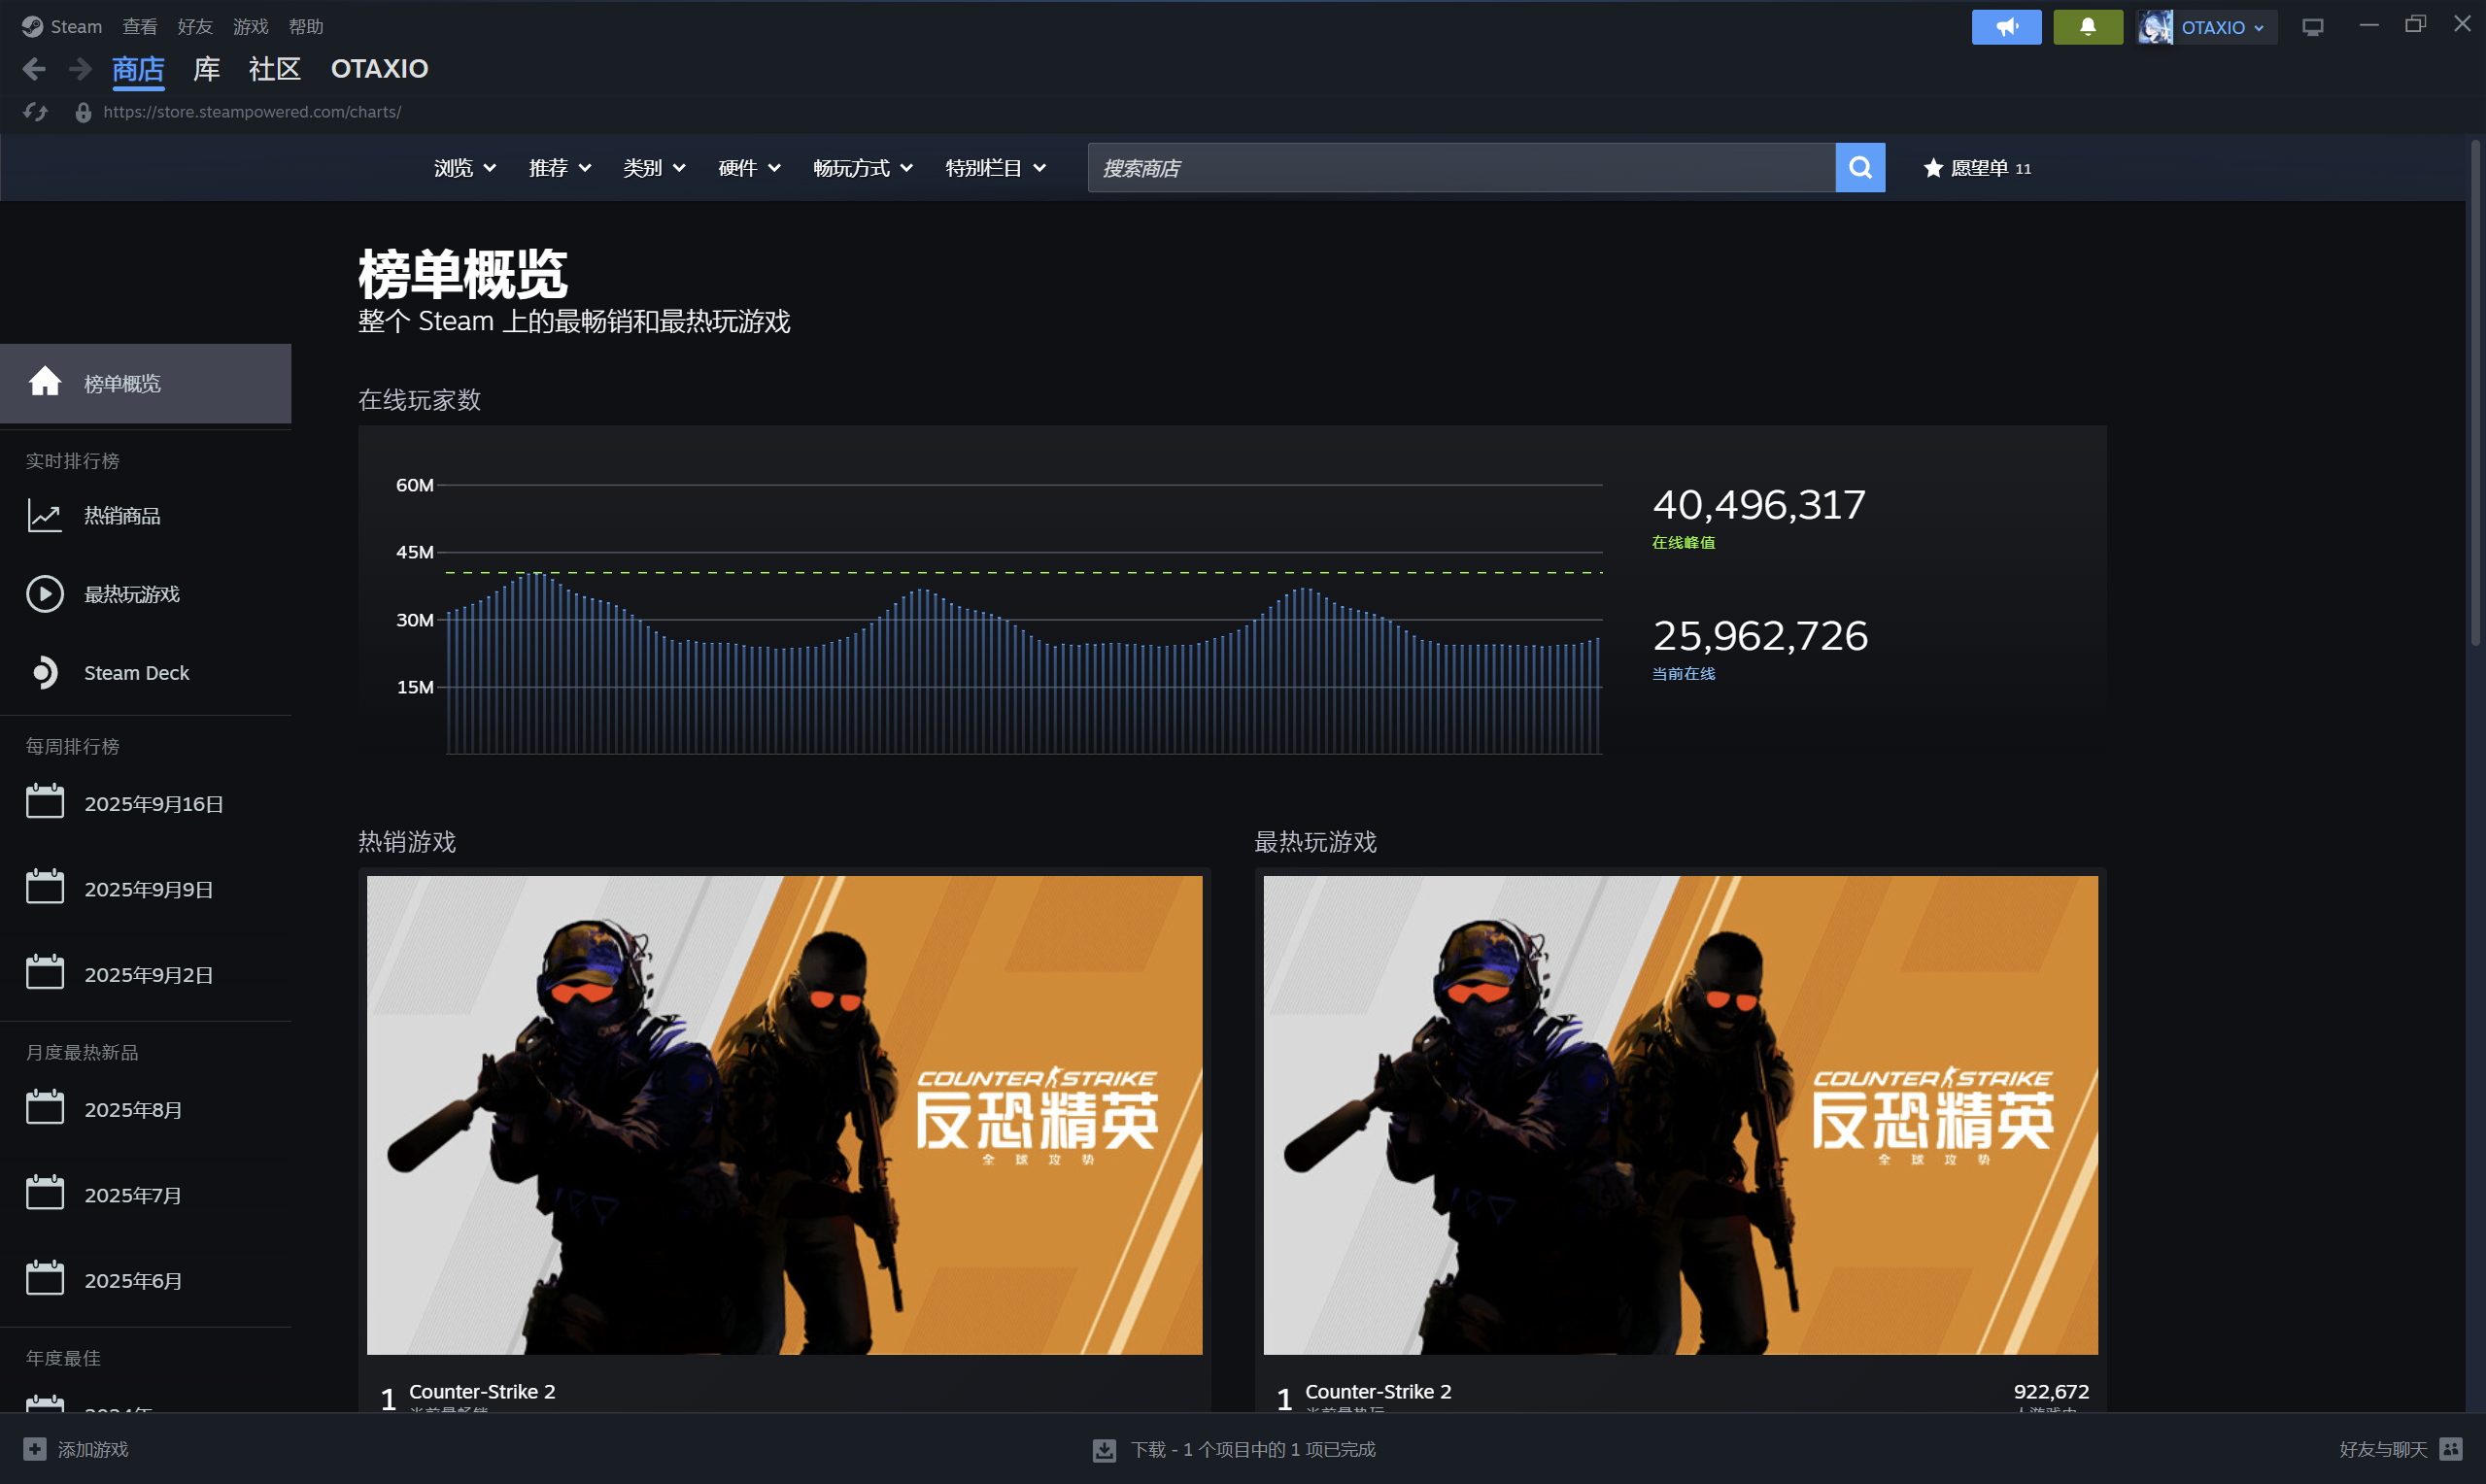
\includegraphics[width=\linewidth]{图/统计数据.png}
                \caption{统计数据}
                \label{fig:统计数据}
            \end{minipage}
        \end{figure}

        \subsubsection{库}
        顾名思义,库就是你买的游戏存储的地方,即游戏仓库。

        将鼠标放在库这个按钮上,你能看到主页,收藏和下载三个分区。
        \begin{itemize}
            \item 主页\ref{fig:库}就是你直接点击进入的模样,左边一列是你库中有的游戏,点击你想要玩的游戏,如果没有下载就点击下载,下载完成后就能点击启动直接游玩了。
            \item 收藏\ref{fig:收藏}本质上是一个分类功能,它能创建类似文件夹的东西,把你认为同类的游戏放在一起。比如笔者这里就是把一些有战斗元素的游戏放在了战斗爽里。
            \item 下载则是显示你游戏下载任务和进度的地方,也可以直接点击整个页面最下面中间的管理下载查看。
        \end{itemize}
        
        \begin{figure}[H]
            \centering
            \begin{minipage}{0.48\textwidth}
                \centering
                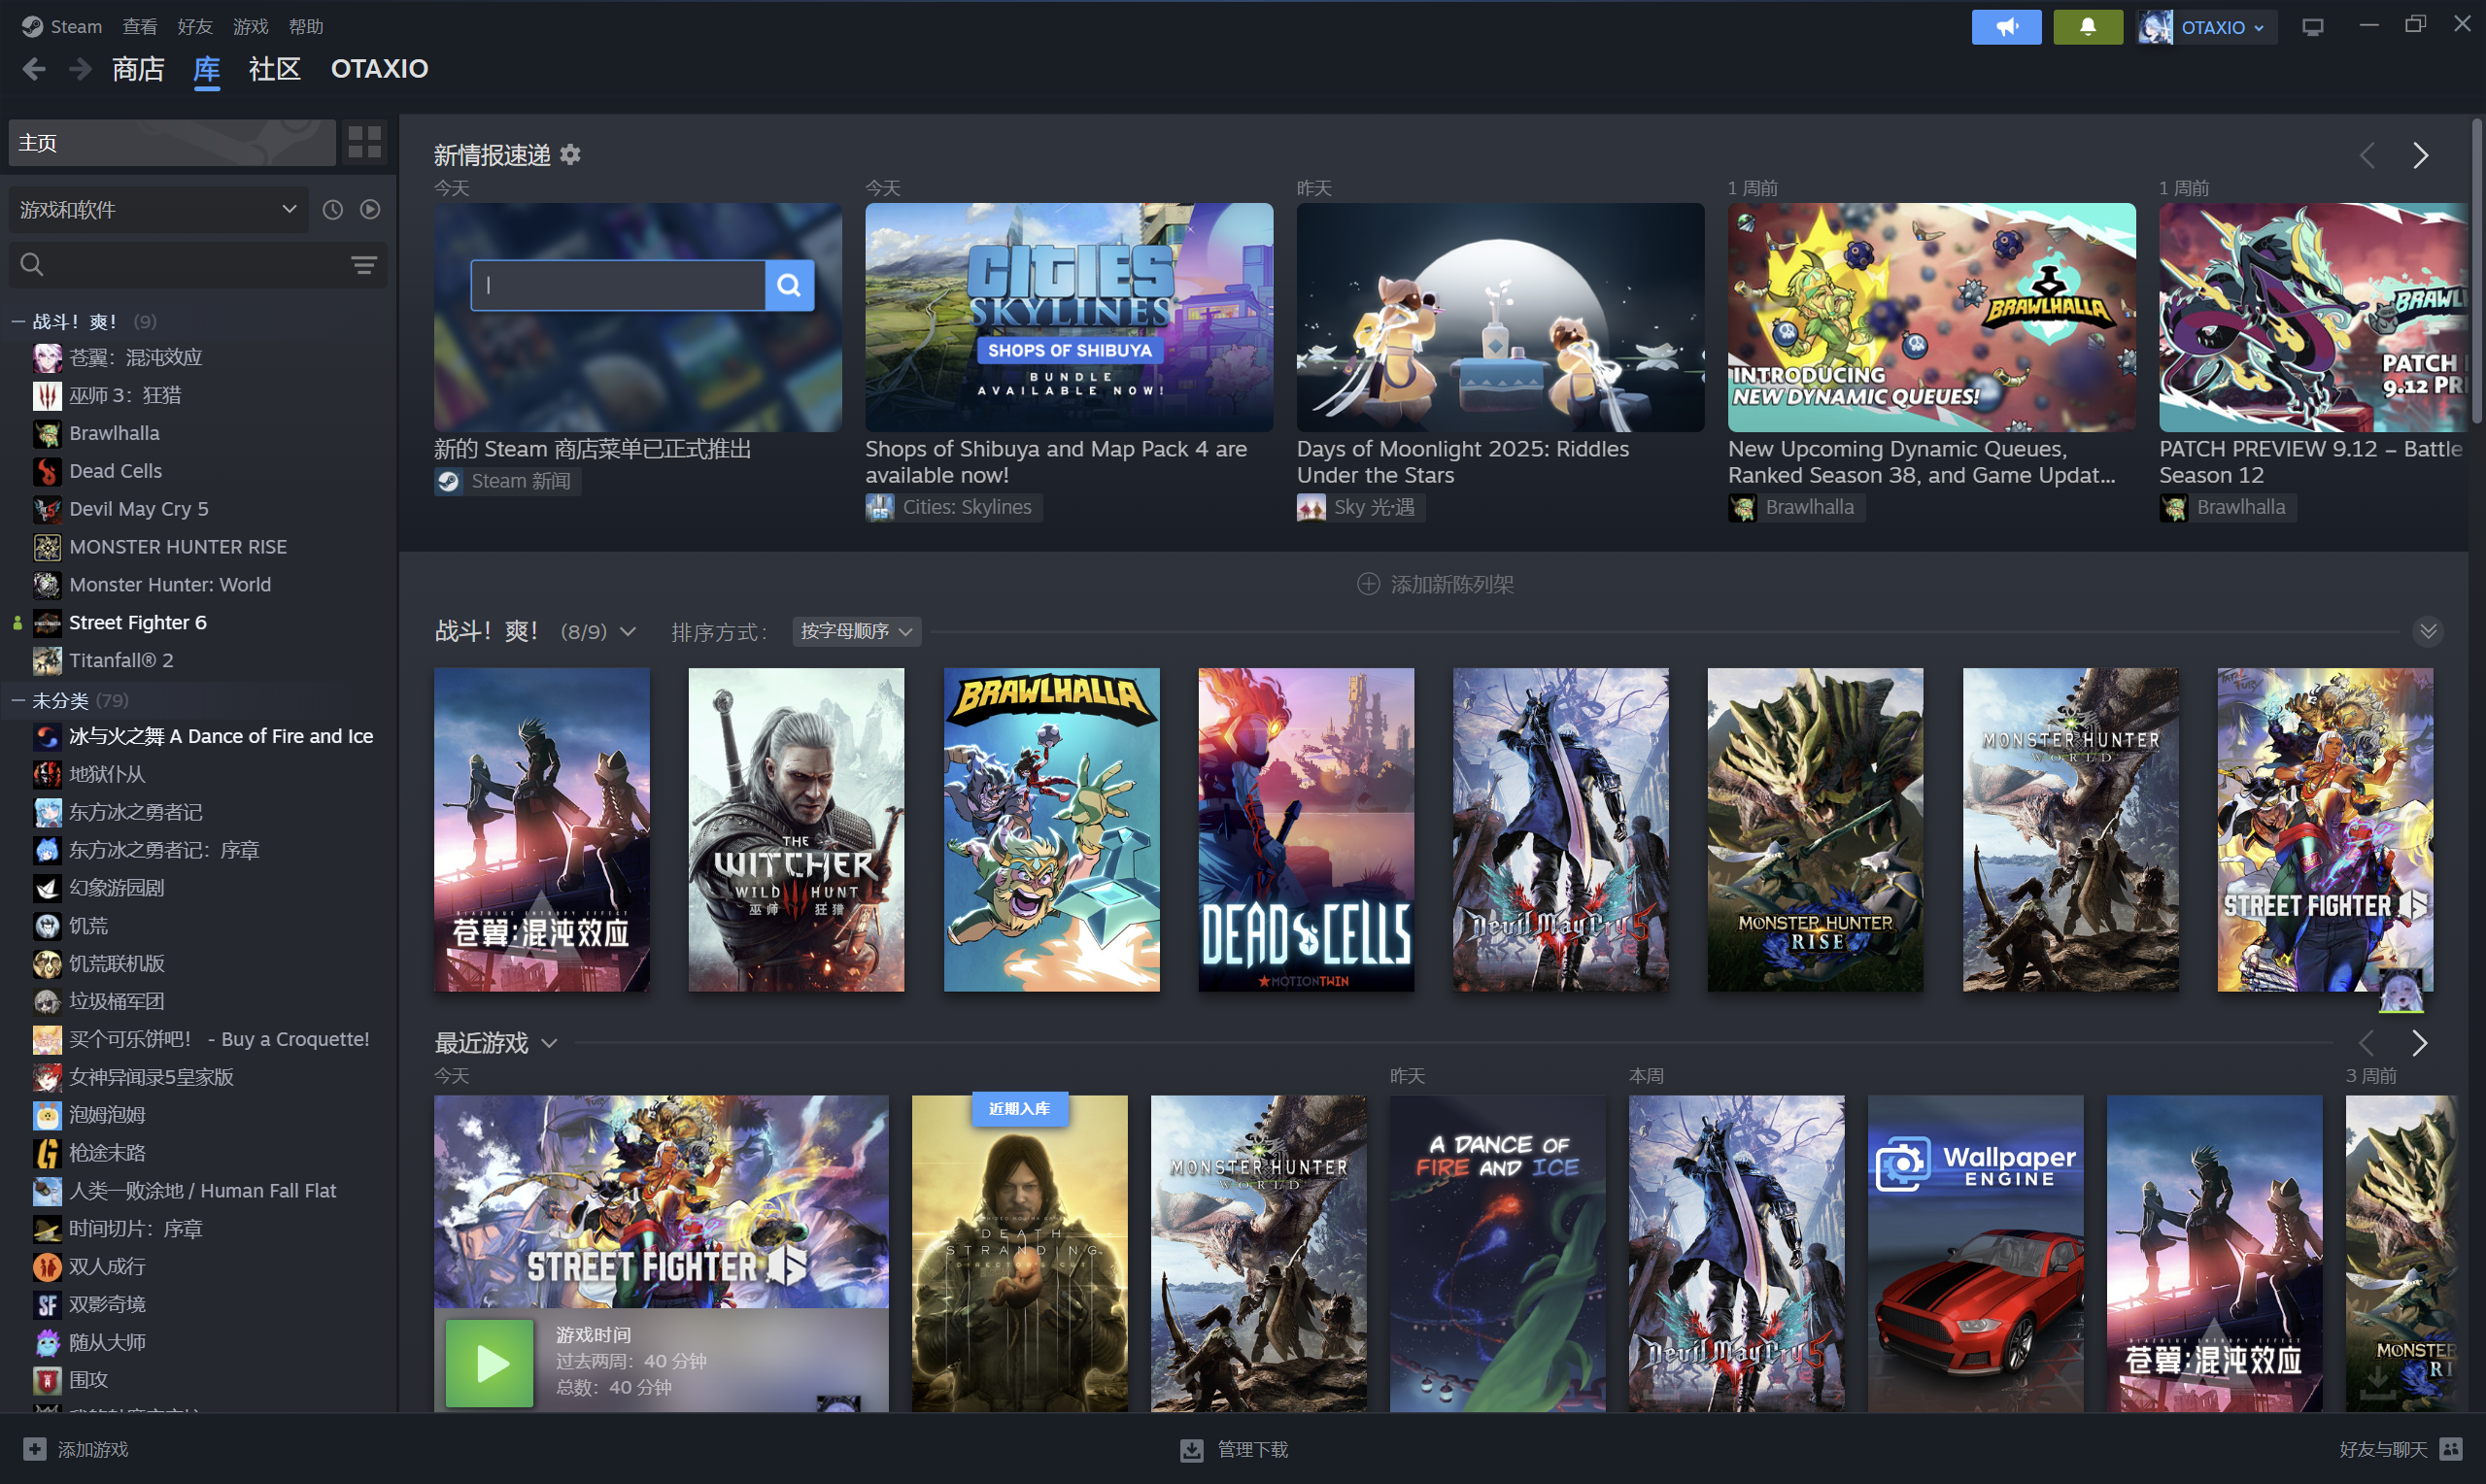
\includegraphics[width=\linewidth]{图/库.png}
                \caption{主页}
                \label{fig:库}
            \end{minipage}
            \hfill
            \begin{minipage}{0.48\textwidth}
                \centering
                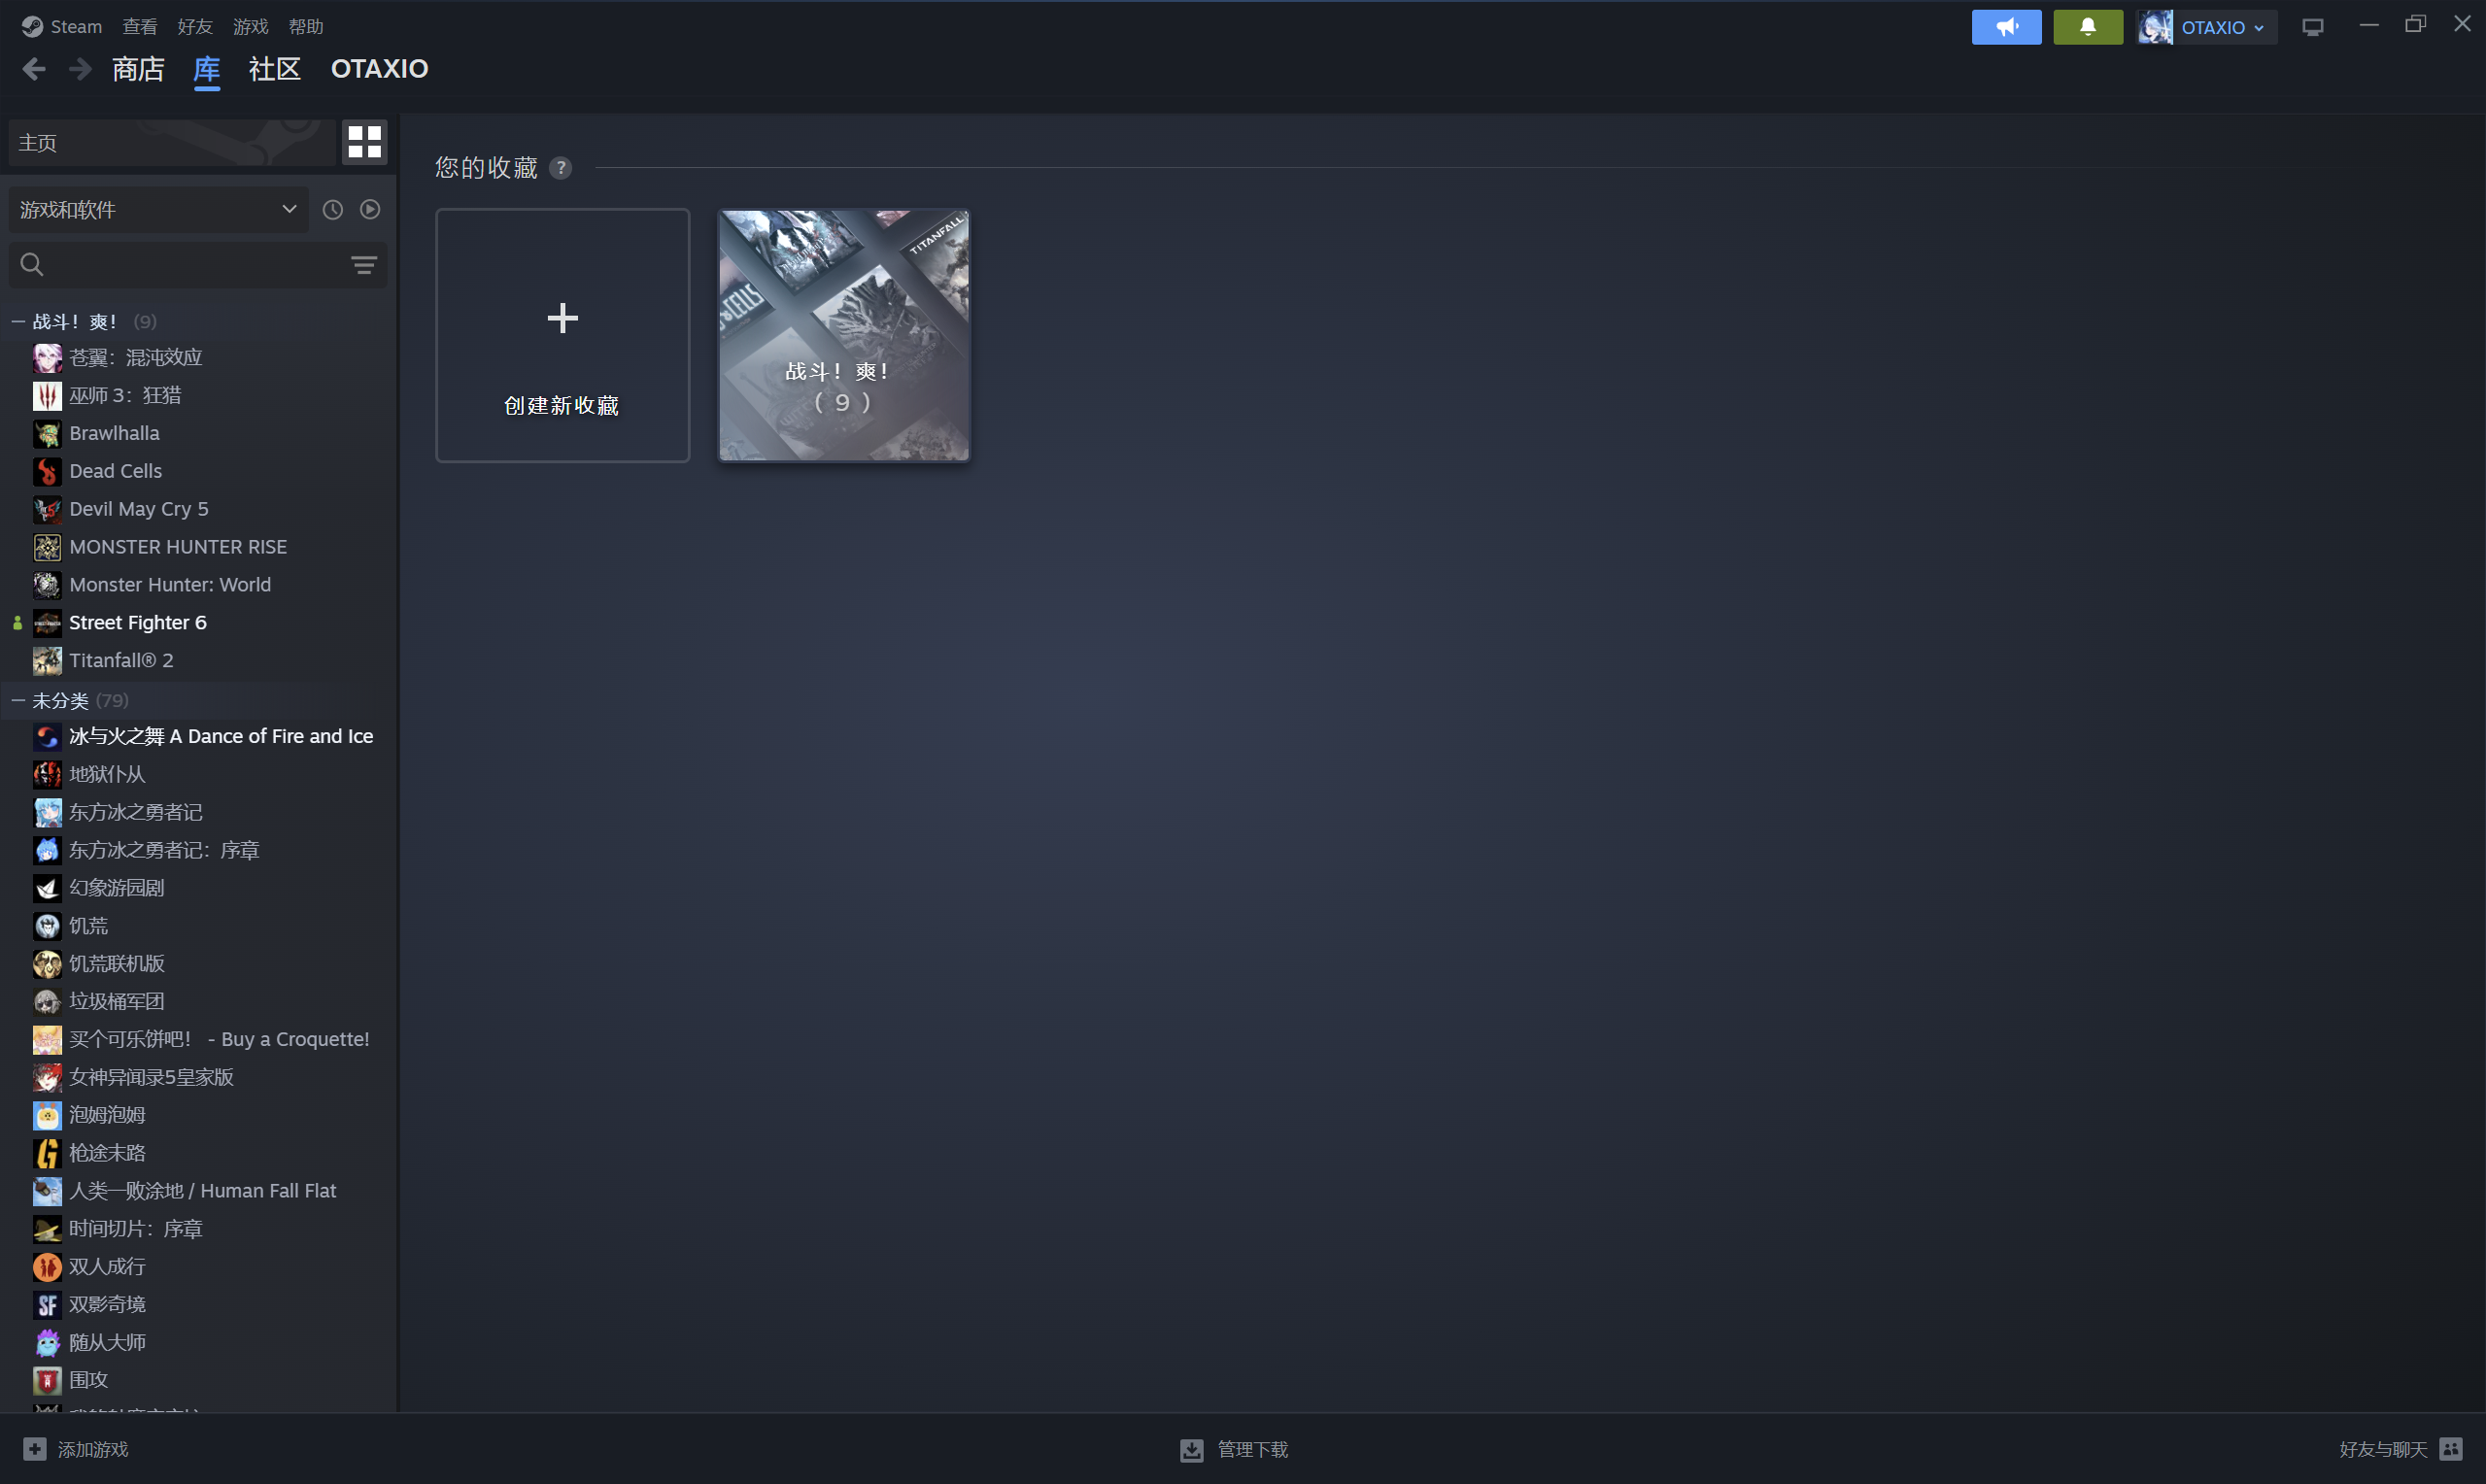
\includegraphics[width=\linewidth]{图/收藏.png}
                \caption{收藏}
                \label{fig:收藏}
            \end{minipage}
        \end{figure}
    
        \subsubsection{社区}
        这一部分主要就是下载mod和进行游戏数字产品交易,笔者对这种功能使用较少,希望有经验的读者可以邮件私信作者,日后补充。

        \subsubsection{个人}
        最后一部分就是个人,即你查看个人资料以及你在Steam的好友,库存,成就等的地方。

        将鼠标放在OTAXIO(你自己的ID)这个按钮上,你能看到动态,个人资料,好友,群组,内容,徽章,库存,Steam回顾八个分区。由于涉及个人隐私,这一部分就不放图片了,细节大家可以自己琢磨。
        \begin{itemize}
            \item 动态一般是查看你以及你好友最近在Steam上的操作,能看到加入愿望单,游戏入库,开始玩游戏,获得成就等。是一个跟好友聊天的契机。
            \item 个人资料则是查看或修改自己对外展示的个人信息,同时,在这个页面右侧可以查看徽章,游戏数量,库存,截图等。
            \item 好友就是你与别人产生联系的地方,觉大多数游戏联机都是添加好友以后更加方便。在这个页面你可以查看好友状态,包括哪些人在玩什么游戏。

            这个页面绝大多数功能都是一看就懂的,但在这之中,有一个功能需要特别提及,就是添加好友\ref{fig:添加好友}这个部分。Steam或许是为了防止机器人诈骗,每个Steam必须至少在Steam商店消费5美元才能添加别人的好友。注意,必须在Steam上消费,使用cdk激活超价值的游戏是不算的(至于cdk是什么在游戏购买部分有讲)。当你有了添加好友的资格,就可以在这个界面输入好友的好友代码并让好友通过申请,或发送快速邀请链接让好友点击(不用电脑有点小麻烦)。
            \item 群组则是像社团一样的存在,大家因为具有共同的特点而聚在一起,可以在群组里交流游戏或其他事物。
            \item 内容这个功能笔者没有使用过,欢迎读者补充。
            \item 徽章属于成就的一种,徽章包含集换式卡牌。卡牌的获取机制比较复杂,简单来说如果你只打游戏是没办法全部收集的,需要跟别人进行交易。这方面笔者经历较浅,欢迎各位读者补充。
            \item 库存则是你在Steam上的数字产品,包括你的集换式卡牌,点数商店购买的装饰。
            \item Steam回顾则是你去年的游戏总结,是Steam为每个账户生成的。可以看到你去年买了哪些游戏,玩了哪些游戏,哪些游戏玩的最久等。
        \end{itemize}
        \begin{figure}[H]
        \centering
        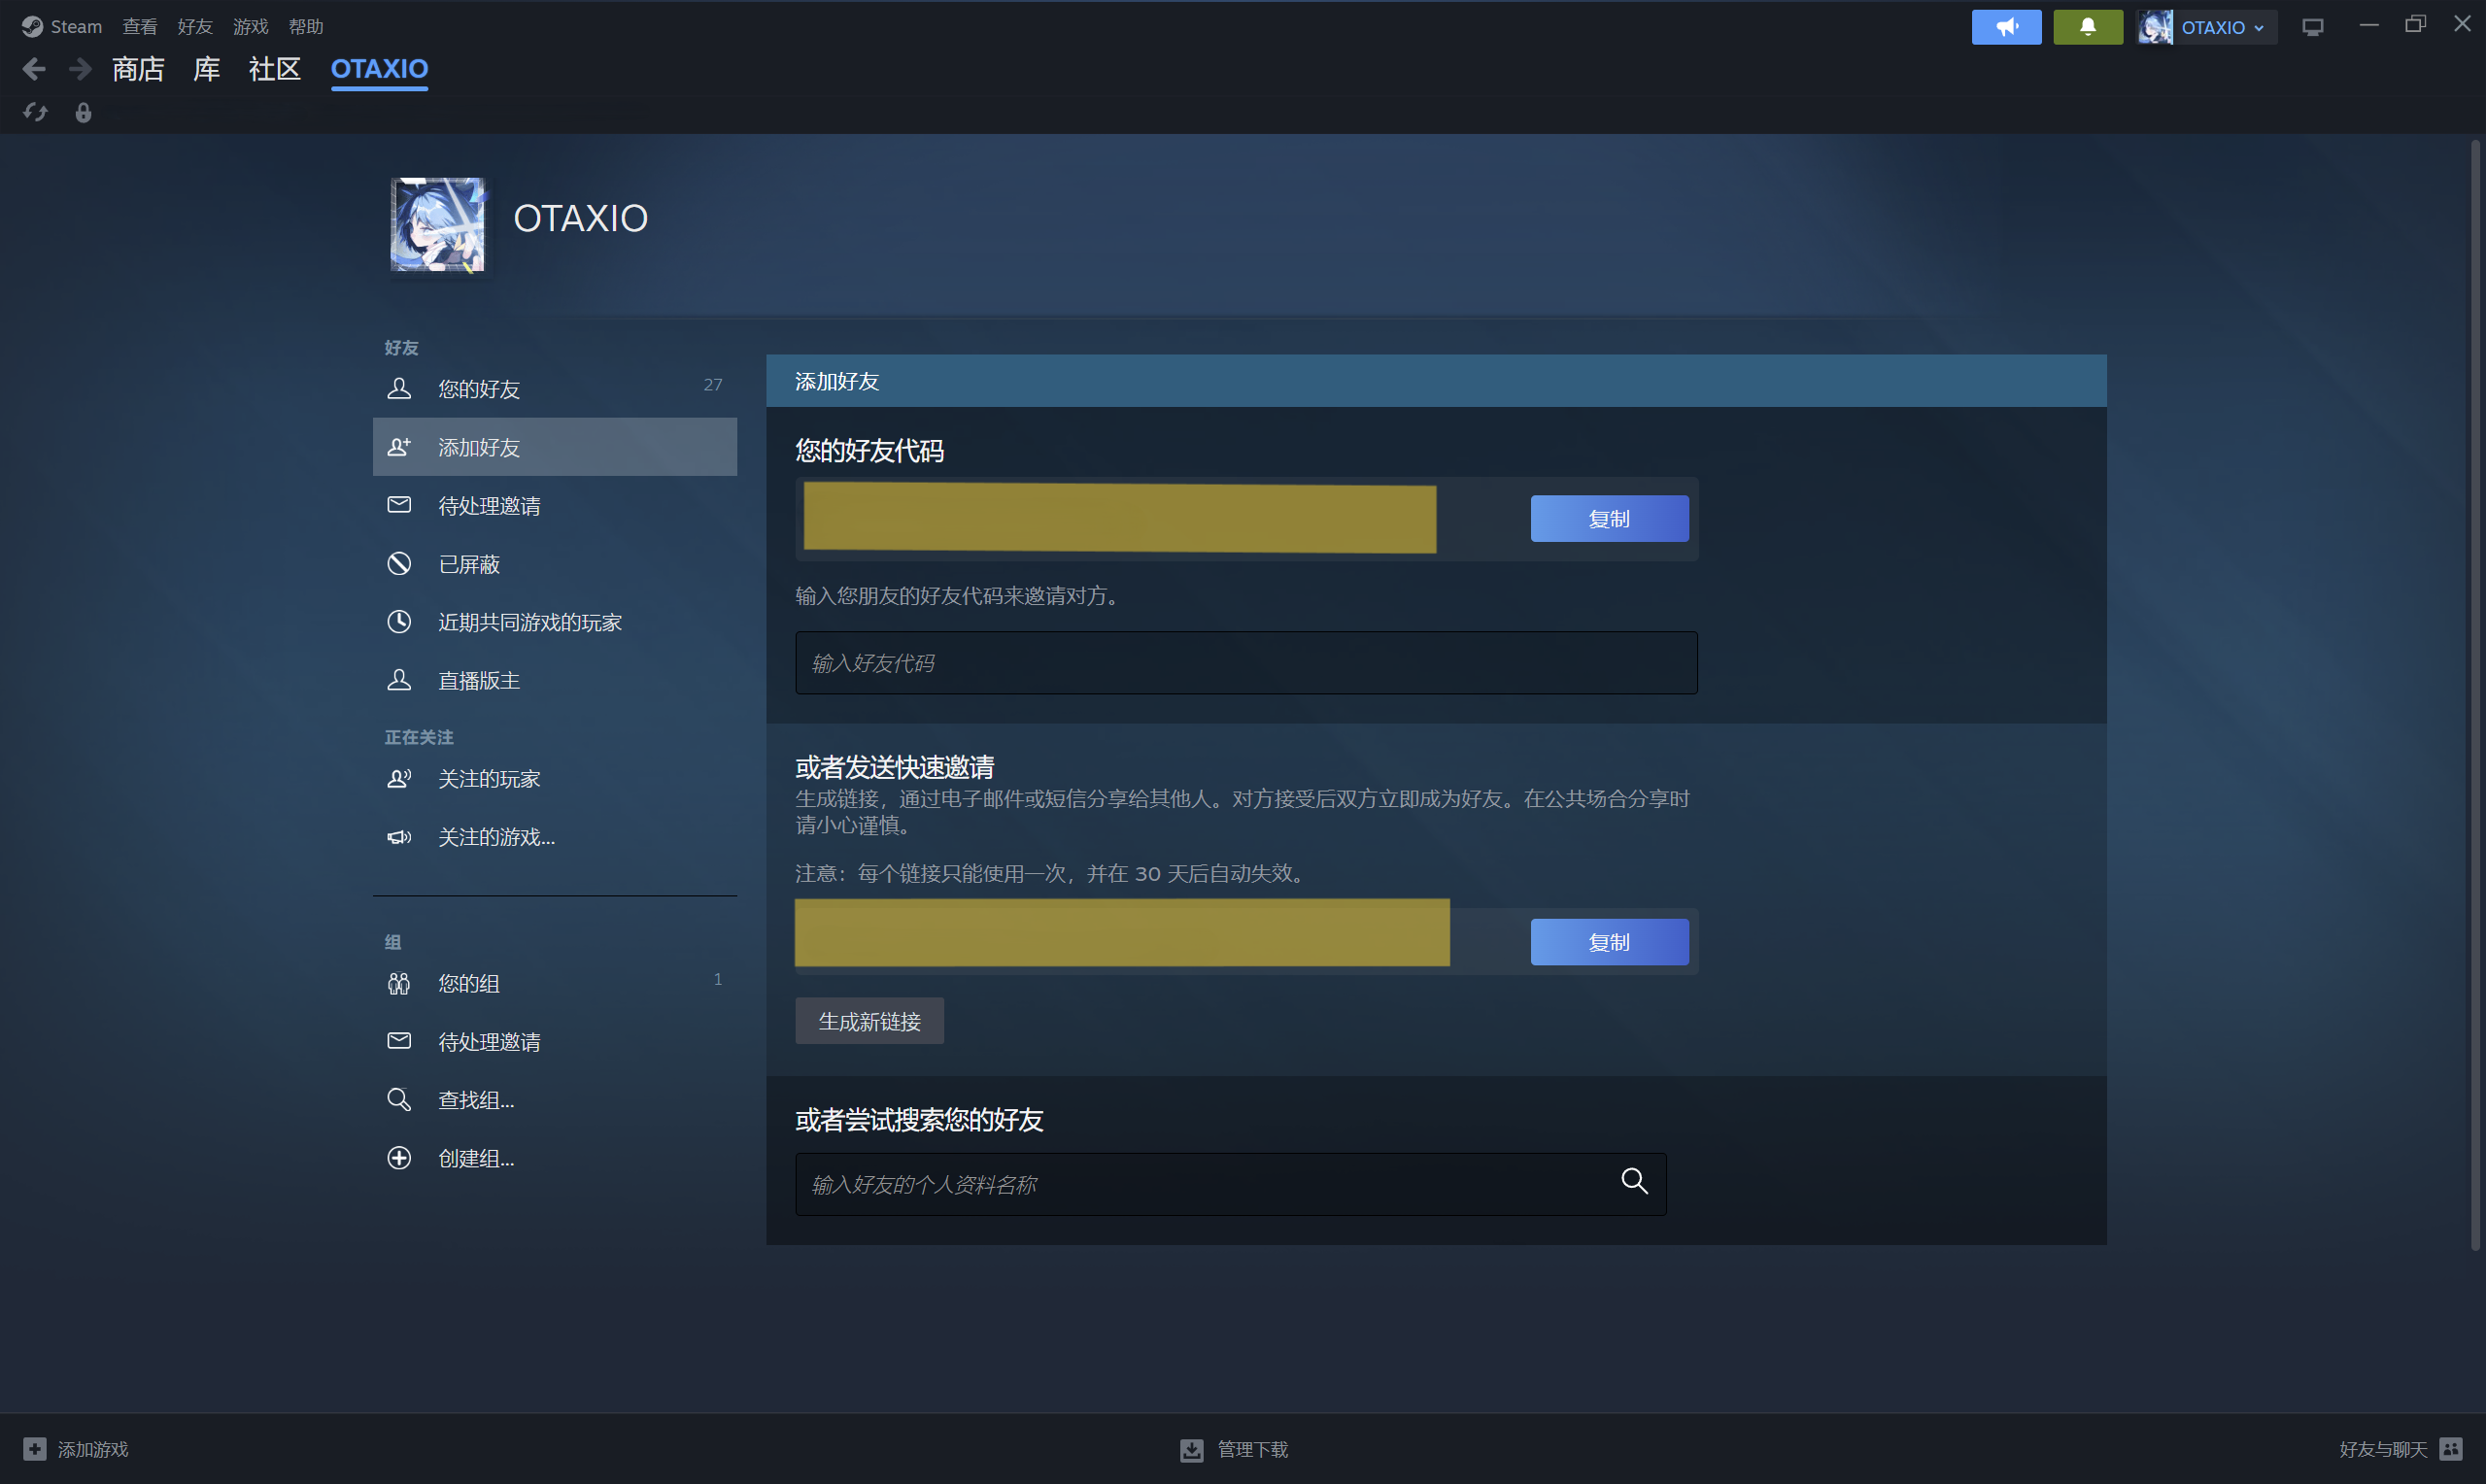
\includegraphics[width=0.7\linewidth]{图/添加好友.png}
        \caption{\label{fig:添加好友}添加好友界面}
        \end{figure}
    \subsection{五小功能}
    左上角除了四个大字号,还有五个小字号的功能\ref{fig:五小功能}。
    \begin{figure}[H]
    \centering
    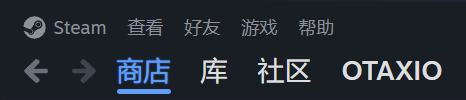
\includegraphics[width=0.7\linewidth]{图/主要四功能.png}
    \caption{\label{fig:五小功能}Steam五小功能}
    \end{figure}
    这五个功能分别是Steam,查看,好友,游戏,帮助。下面笔者将详细介绍这五小功能。(虽然笔者称其为五小功能,只是说明其字号较小,而并不是说这五个按钮用处不大)
        \subsubsection{Steam}
        这个按钮主要控制你Steam的运行,有更换账号...,退出...,进入离线模式,检查Steam客户端更新,还原游戏备份,设置和退出。
        \begin{itemize}
            \item 更换账号就是先退出Steam登录,再跳出登录界面。
        \end{itemize}

\subsection{Good luck!}

We hope you find Overleaf useful!
